%
%
% UCSD Doctoral Dissertation and Masters Thesis Template
% -----------------------------------
% https://github.com/ucsd-thesis/ucsd-thesis
%
%
% ----------------------------------------------------------------------
% WARNING: 
%
%   This template has not endorsed by OGS or any other official entity.
%   The official formatting guide can be obtained from OGS.
%   It can be found on the web here:
%   http://grad.ucsd.edu/_files/academic-affairs/Dissertations_Theses_Formatting_Manual.pdf
%
%   No guarantee is made that this LaTeX class conforms to the official UCSD guidelines.
%   Make sure that you check the final document against the Formatting Manual.
%  
%   That being said, this class has been routinely used for successful 
%   publication of doctoral theses.  
%
%   The ucsd.cls class files are valid for doctoral dissertations and
%    masters theses.
%
% ----------------------------------------------------------------------
% GETTING STARTED:
%
%   Lots of information can be found on the project wiki:
%   http://code.google.com/p/ucsd-thesis/wiki/GettingStarted
%
%
%   To make a pdf from this template use the command:
%     pdflatex template
%
%
%   To get started please read the comments in this template file 
%   and make changes as appropriate.
%
%   If you successfully submit a thesis with this package please let us
%   know.
%
%
% ----------------------------------------------------------------------
% KNOWN ISSUES:
%
%   Currently only the 12pt size conforms to the UCSD requirements.
%   The 10pt and 11pt options make the footnote fonts too small.
%
%
% ----------------------------------------------------------------------
% HELP/CONTACT:
%
%   If you need help try the ucsd-thesis google group:
%   http://groups.google.com/group/ucsd-thesis
%
%
% ----------------------------------------------------------------------
% BUGS:
%
%   Please report all bugs at:
%   https://github.com/ucsd-thesis/ucsd-thesis/issues
%
%
% ----------------------------------------------------------------------
% More control of the formatting of your thesis can be achieved through
% modifications of the included LaTeX class files:
%
%   * ucsd.cls    -- Class file
%   * uct10.clo   -- Configuration files for font sizes 10pt, 11pt, 12pt
%     uct11.clo                            
%     uct12.clo
%
% ----------------------------------------------------------------------



% Setup the documentclass 
% default options: 12pt, oneside, final
%
% fonts: 10pt, 11pt, 12pt -- are valid for UCSD dissertations and theses.
% sides: oneside, twoside -- note that two-sided theses are not accepted 
%                            by OGS.
% mode: draft, final, lulu -- 
%                            draft mode switches to single spacing, 
%                            removes hyperlinks, and places a black box
%                            at every overfull hbox (check these before
%                            submission).
%
%                            lulu mode prints to 6x9, single spacing, and ready for 
%                            double-sided printing.
%
% degree: phd, masters --
%                            this changes the template to conform to (dissertation or thesis needs)
%
% chapterheads            -- Include this if you want your chapters to read:
%                              Chapter 1
%                              Title of Chapter
%
%                            instead of
%                              1 Title of Chapter
%
% en                      (default) you can add translations to languages/[lang].tex,
%                           then switch languages.
%
\documentclass[12pt,final,masters,chapterheads]{ucsd}  % or masters instead of phd


% Include all packages you need here.  
% Some standard options are suggested below.
%
% See the project wiki for information on how to use 
% these packages. Other useful packages are also listed there.
%
%   http://code.google.com/p/ucsd-thesis/wiki/GettingStarted



%% AMS PACKAGES - Chances are you will want some or all 
%    of these if writing a dissertation/thesis that includes equations.
%  \usepackage{amsmath, amscd, amssymb, amsthm}
\usepackage{amsmath, amscd, amssymb, amsthm}

%% GRAPHICX - This is the standard package for 
%    including graphics for latex/pdflatex.
%\usepackage{scrextend}
%\usepackage{pslatex}
%\usepackage{graphicx}


%% SUBFIG - Use this to place multiple images in a
%    single figure.  Subfig will handle placement and
%    proper captioning (e.g. Figure 1.2(a))
% \usepackage{subfig}

%% TIMES FONT - replacements for Computer Modern
%%   This package will replace the default font with a
%%   Times-Roman font with math support.
\usepackage[T1]{fontenc}
\usepackage{mathptmx}

%% INDEX
%   Uncomment the following two lines to create an index: 
% \usepackage{makeidx}
% \makeindex
%   You will need to uncomment the \printindex line near the
%   bibliography to display the index.  Use the command
% \index{keyword} 
%   within the text to create an entry in the index for keyword.
%   To compile a LaTeX document with an index the 'makeindex'
%   command will need to be run.  See the wiki for more details.



%% CITATIONS
% Sets citation format
% and fixes up citations madness
\usepackage{microtype}  % avoids citations that hang into the margin

%% String comparisons
\usepackage{pdftexcmds}

%% FOOTNOTE-MAGIC
% Enables footnotes in tables, re-referencing the same footnote multiple times.
\usepackage{footnote}
\makesavenoteenv{tabular}
\makesavenoteenv{table}


%% TABLE FORMATTING MADNESS
% Enable all sorts of fun table tricks
\usepackage{rotating}  % Enables the sideways environment (NCPW)
\usepackage{array}  % Enables "m" tabular environment http://ctan.org/pkg/array
\usepackage{booktabs}  % Enables \toprule  http://ctan.org/pkg/array


%% HYPERLINKS
%   To create a PDF with hyperlinks, you need to include the hyperref package.
%   THIS HAS TO BE THE LAST PACKAGE INCLUDED!
%   Note that the options plainpages=false and pdfpagelabels exist
%   to fix indexing associated with having both (ii) and (2) as pages.
%   Also, all links must be black according to OGS.
%   See: http://www.tex.ac.uk/cgi-bin/texfaq2html?label=hyperdupdest
%   Note: This may not work correctly with all DVI viewers (i.e. Yap breaks).
%   NOTE: hyperref will NOT work in draft mode, as noted above.
\usepackage[colorlinks=true, pdfstartview=FitV, 
            linkcolor=black, citecolor=black, 
            urlcolor=black, plainpages=false,
            pdfusetitle, pdfpagelabels]{hyperref}
\urlstyle{same}
\usepackage{bookmark}

\usepackage{xcolor}
\newcommand\todo[1]{\textcolor{red}{#1}}

\usepackage{float}

\begin{document}

%% FRONT MATTER
%
%  All of the front matter.
%  This includes the title, degree, dedication, vita, abstract, etc..
%  Modify the file template_frontmatter.tex to change these pages.
%
%
% UCSD Doctoral Dissertation Template
% -----------------------------------
% http://ucsd-thesis.googlecode.com
%
%


%% REQUIRED FIELDS -- Replace with the values appropriate to you

% No symbols, formulas, superscripts, or Greek letters are allowed
% in your title.
\title{ALE Analytics: A Software Pipeline and Web Platform for the Analysis of Microbial Genomic Data from Adaptive Laboratory Evolution Experiments}

\author{Patrick Phaneuf}
\degreeyear{\the\year}
\campus{San Diego}  % used as: University of California, \campus


% Master's Degree theses will NOT be formatted properly with this file.
\degreetitle{\thedegree}

\field{Computer Science and Engineering}
% \specialization{Anthropogeny}  % If you have a specialization, add it here

\chair{Professor Bernhard Palsson}
% Uncomment the next line iff you have a Co-Chair
% \cochair{Professor Cochair Semimaster}
%
% Or, uncomment the next line iff you have two equal Co-Chairs.
%\cochairs{Professor Chair Masterish}{Professor Chair Masterish}

%  The rest of the committee members  must be alphabetized by last name.
\othermembers{
Professor Vineet Bafna\\
Professor Pavel Pevzner\\
}
 \ifnum\pdfstrcmp{\@degree}{masters}=0 %
    \numberofmembers{3} % |chair| + |cochair| + |othermembers|
\else
    \numberofmembers{4} % |chair| + |cochair| + |othermembers|
\fi

%% START THE FRONTMATTER
%
\begin{frontmatter}

%% TITLE PAGES
%
%  This command generates the title, copyright, and signature pages.
%
\makefrontmatter


%% SETUP THE TABLE OF CONTENTS
%
\tableofcontents
\listoffigures  % Comment if you don't have any figures
\listoftables   % Comment if you don't have any tables


%% ABSTRACT
%
%  Doctoral dissertation / thesis abstracts should not exceed 350 words.
%   The abstract may continue to a second page if necessary.
%
\begin{abstract}
%Adaptive Laboratory Evolution (ALE) is a tool for studying biological molecular mechanisms and evolutionary dynamics through coupling with whole genome sequencing. Academic and industrial labs involved in the study of microbial evolution and metabolic engineering use ALE methodologies in their research for exploring adaptive mutations \cite{ASM:/content/journal/microbe/10.1128/microbe.6.69.1}. These labs build custom post-processing and computational pipelines for the analysis of the ALE genomic output, though ALE methodologies often include the same fundamental steps to interrogate the evolutionary trajectory of the organisms under study. This thesis will detail the strategies and computational tools used in the ALE project pipeline executed by UCSD's Systems Biology Research Group (SBRG) and describe a system for compiling and analyzing ALE results. This thesis can contribute to the domain of ALE methodologies by detailing an approach to the computational analysis of ALE experiments, will propose a method for hypothesizing key mutations and will explore global trends for all ALE experiment data accumulated. These computational tools and protocols to identifying key mutations and global trends will be leveraged, implemented and evaluated in our ALE Analytics software pipeline and web platform. We therefore hypothesize that we can leverage existing ALE foundational technologies and methodologies to develop a bioinformatics system that will accurately predict the key mutations of ALE experiments and provide context on global mutational trends and correlated experimental conditions.
Adaptive Laboratory Evolution (ALE) methodologies are used for studying microbial adaptive mutations that optimize host metabolism. The Systems Biology Research Group (SBRG) at the University of  California, San Diego, has implemented high-throughput ALE experiment automation that enables the group to expand their experimental evolutions to scales previously infeasible with manual workflows. The data generated by the high-throughput automation now requires a post-processing, content management and analysis framework that can operate on the same scale. We develop a software system which solves SBRG's specific ALE big data to knowledge challenges. The software system is comprised of a post-processing software protocol for quality control and feedback, a software framework and database for data consolidation and a web platform for reports and automated analysis. The automated analysis is evaluated against published ALE experiment results and maintains an average recall of 89.6\%, an average precision of 71.2\% and identifies key mutations in genes \textit{wecA} and \textit{yjiT} not included in the published work. The consolidation of all ALE experiments into a unified resource has enabled the development of ALE Analytics features that compare key mutations across multiple experiments. These features find the genomic regions \textit{rph}, \textit{hns-tdk}, \textit{rpoB}, \textit{rpoC} and \textit{pykF} mutated in more than one ALE experiment published by SBRG. We reason that leveraging this software system relieves the bottleneck in ALE experiment analysis and generates new data mining opportunities for research in understanding system-level mechanisms that govern adaptive evolution.
\end{abstract}


\end{frontmatter}




%% DISSERTATION

% A common strategy here is to include files for each of the chapters. I.e.,
% Place the chapters is separate files: 
%   chapter1.tex, chapter2.tex
% Then use the commands:
%   \include{chapter1}
%   \include{chapter2}
%
% Of course, if you prefer, you can just start with
%   \chapter{My First Chapter Name}
% and start typing away.  
\chapter{Introduction}

% * <pphaneuf@eng.ucsd.edu> 2016-10-13T02:09:24.496Z:
%
% TODO: re-write introduction to better fit the final thesis content.
%
% ^.

% * <pphaneuf@eng.ucsd.edu> 2016-10-13T02:37:41.790Z:
%
% TODO: Somewhere within the paper, describe the infrastructure and features necessary (filtering, server, HTTPs, search gene structure, etc).
%
% ^.

% * <pphaneuf@eng.ucsd.edu> 2016-10-16T01:24:35.111Z:
%
% TODO: Need to describe why we care about experimental evolution! Mentioned reasons in abstract, but didn't give explanation. This will lead us into background, challenges, etc.
%
% ^ <pphaneuf@eng.ucsd.edu> 2016-10-18T21:28:48.339Z:
%
% Can study the fundamental mechanism of evolution and DNA.
%
% ^.

Adaptive Laboratory Evolution (ALE) experiment
Include statement on academia and industry leveraging ALE.

\chapter{Motivation and Specific Aims}

% * <pphaneuf@eng.ucsd.edu> 2016-08-13T21:50:16.076Z:
%
% "Tightly controlled experimental conditions allowed selection based on exponential-phase growth rate, yielding strains that uniformly converged toward a similar phenotype along distinct genetic pathways."
%
% ^ <pphaneuf@eng.ucsd.edu> 2016-08-13T21:55:53.371Z:
%
% -42C
%
% ^.

% * <pphaneuf@eng.ucsd.edu> 2016-08-13T22:05:08.401Z:
%
% ALE Experiments often involve parallel adaptive evolution to study of multiple mutational trajectories towards a similar phenotype
%
% ^.

% * <pphaneuf@eng.ucsd.edu> 2016-08-13T21:54:45.239Z:
%
% "Adaptive laboratory evolution, or ALE, has developed over the years into a potent tool for biological discovery and engineering (Dragosits and Mattanovich 2013)" -42C
%
% ^.

\section{Background}
\subsection{ALE Experiment}

% * <pphaneuf@eng.ucsd.edu> 2016-08-13T22:16:30.308Z:
%
% Describe ALE, Flask, Isolate, Replicate setup within the context of an ALE Experiment.
%
% ^.

% * <pphaneuf@eng.ucsd.edu> 2016-10-18T00:37:54.248Z:
%
% TODO: should I mention GEMs?
%
% ^.

The foundational work to which this thesis builds on are the ALE experimental wet lab methodologies. Beginning with a well known starting strain, an ALE experiment is commonly executed by serially passing a selected cell culture to a fresh flask of media (Figure \ref{fig:ale_experiment_samples}), enabling the particular strain passed to continue evolving under the experimental controls. The selection of cells to pass on to the next flask is often based on population size since we assume that the most adapted strain population will outgrow their competition. ALE experiments can also involve replicate ALEs, which are identical experimental evolutions that execute in parallel. This approach reveals additional mutational data on the dynamics of adaptation and evolution for an organism and reveal a convergence of adaptations across multiple ALEs \cite{sys_bio_book}.

\begin{figure}[h!]
  \caption{\textbf{A} An illustration of an ALE from an ALE experiment where both a clonal and population sample are isolated from a midpoint flask. The petri dish illustrates a the streaking out of a colony for capturing clonal samples. The Eppendorf tube illustrates a population sample of possible heterogeneous strains. \textbf{B} An illustration of how an ALE experiment can have many ALEs, flask and isolates and how they are associated with each other.}
  \centering
  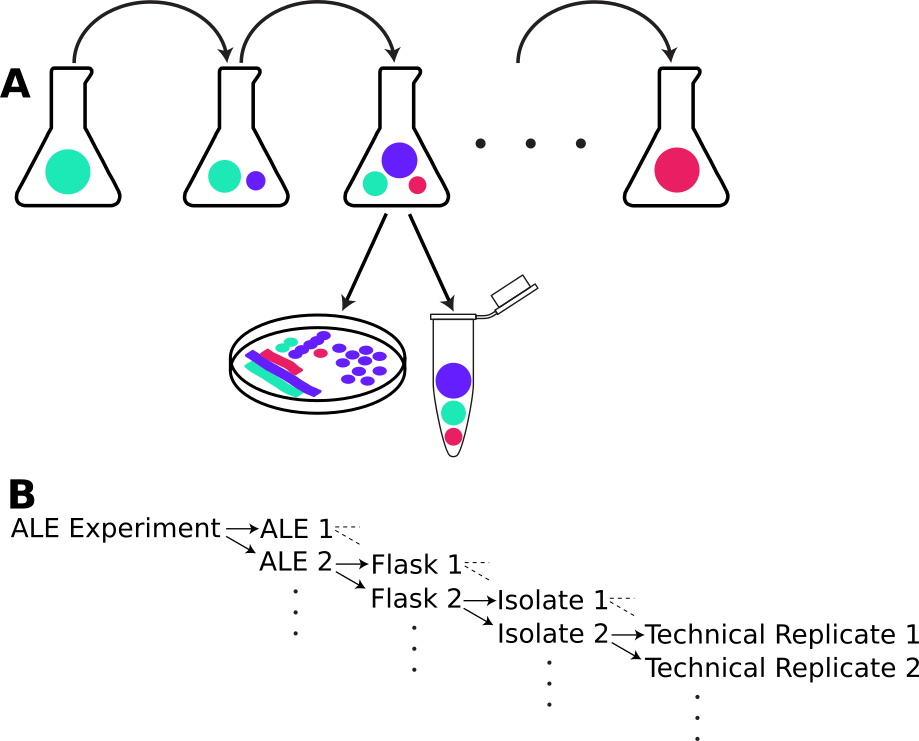
\includegraphics[width=1\textwidth]{ale_experiment_samples.png}
  \label{fig:ale_experiment_samples}
\end{figure}

% * <pphaneuf@eng.ucsd.edu> 2016-10-20T21:11:49.690Z:
%
% TODO: in the above figure, insert a coinciding figure (therefore have figure A and B) which describes the a mapping of ALEs -> Flasks -> Isolates -> Replicates.
%
% ^.

The output of an ALE experiment are population or clonal isolates which were derived from the original strain and additionally include mutations according to the environmental stresses introduced in the ALE experiment. This output is then processed by additional foundational technologies leveraged with ALE: the DNA sequencer and mutation identifying software. In the ALE Analytics software pipeline, the output sample to be analyzed is sequenced, typically by an Illumina MiSeq small genome sequencer, and resequenced primarily using the \textit{Breseq} computational pipeline. \textit{Breseq}'s resequencing process aligns all of the DNA reads to a provided genome reference and reports single-nucleotide mutations, point insertions and deletions, large deletions, and new junctions according to the differences in the aligned reads and the reference genome \cite{breseq_paper}.

Generally, researchers compare the mutations from each ALE's endpoint samples to identify genomic regions with multiple alleles. If a researcher sequenced midpoint samples for ALEs, an ALE's mutations can be organized in chronological order to identify mutations that fix. The mutations that are involved in multiple alleles of a genomic region or are shown to fix from midpoint to endpoint samples are considered the \textit{key mutation} sets and are investigated for their possible fitness benefit according to the genomic region they affect.

% The ALE Analytics web platform leverages these fundamental technologies by importing the Breseq mutation predictions into a database and implementing a user web interface to enable the querying and curation of mutational trends. Currently, no other work has been published on the practical methodologies for analyzing ALE output; this thesis would be the first to publish on the concrete techniques and technologies used in interpreting ALE results en masse. This software pipeline and web platform will also accelerate the biological decision making necessary to leverage causal mutation for industrial and medical applications.

\subsection{ALE Machine}

ALE methodologies are becoming increasingly popular for their potential in revealing novel discoveries on evolution and designing organisms, though their execution is often labor intensive and requires significant run-time. To impose a balance on the required labor, many ALE experiments are designed to allow for approximately 24 hours between sessions.

Executing manual ALE experiments often restricts the possible experimental parameters according to the feasible amount of experiment monitoring. Current technologies in automation can be leveraged to automate many of the ALE processes, therefore alleviating these restrictions. Automation additionally can contribute to the consistency of the ALE processes, better ensuring that results are due to experimental conditions and not inconsistencies in experiment protocol execution. Finally, automation can enable the scale of an experiment to be greatly expanded at a much lower cost of effort to the experimentalists. This results in the potential for a larger amount of data to be generated on an ALE experiment, providing more resolution on the evolutions. These possible benefits have lead to the Systems Biology Research Group to development an ALE automation platform, referred to as an \textit{ALE Machine} \cite{ryan_thesis}.

The \textit{ALE Machine} platform was designed to eliminate many of the constraints that manual ALE experiments are subjected to, therefore enabling larger ALE experiments with more consistent data. These outcomes are a boon to those studying evolution and encourage experimentalists to leverage ALE methodologies to better explore the dynamics of evolution.

\section{Challenges}

% * <pphaneuf@eng.ucsd.edu> 2016-10-18T00:57:23.628Z:
% 
% NOTE: Be abstract in the description of the issues; the specific problems we were experience and our solution should be elaborated on later in the results of each aim with a case study.
% 
% ^.

The potential for more diverse and greater scale ALE experiments enabled by the \textit{ALE Machine}'s automation exacerbates existing challenges and introduces new challenges. The following is an itemization and description of each challenges considered for this thesis.

\subsection{Post-Processing Protocol}

Many tools exist for the quality control of sequencing data and the identification of mutations. Each tool comes with an inherent set of strengths and weaknesses. For the case of our ALE experiment operations, consistency in the format and quality of our result are primary priorities. %, therefore a tool-set needed to be established and employed in our ALE experiment post-processing pipeline.

%More experiments translates to a higher probability of quality issues with any of the steps in the ALE experiment wet lab methodologies. Quality control measures are employed by most who work with sequencing data, though the process and tool-set employed by each individual may vary. For our ALE experiment post-processing, a quality control process needed to be established to ensure consistent ALE experiment result quality.

\subsection{Experiment Data Consolidation Effort}

As the scale of an ALE experiment grows, so too does the effort necessary to curate the data of the experiment's samples into a report that describes the ALE experiment's mutation lineages. These manual curations are additionally prone to human error, which is more likely to occur with larger experiments.

\subsection{Experiment Analysis Effort and Consistency}

The issues of data consolidation with larger scale experiment also manifest with the analysis of the experiment results. The \textit{key mutation} analysis of experiments may be inconsistent between investigators. \textit{Key mutations} may be excluded from the analysis of the results depending on the amount of experience of an ALE experimentalist. Different methods of reporting experiment results may be used between experimentalists, therefore making the comparison of different ALE experiments more difficult.

\subsection{Results Accessibility}

% * <pphaneuf@eng.ucsd.edu> 2016-10-18T01:40:51.327Z:
%
% TODO: solution is unification of all results in a globally accessible location.
%
% ^.

ALE experiments often involve multiple experimentalists and collaborators. The input of many collaborators may be necessary to fully capture and understand the results of an experiment. These collaborators may be local or remotely located. The logistics of sharing results is often challenging between local collaborators and more problematic between remote collaborators. This is especially true when comparing multiple experiment results from both current and past ALE experiments.


\section{Specific Aims}

We defined a specific set of aims that would lead to solutions to these challenges. These aims are as follows:

\subsection{Aim 1: Establish a Post-Processing Pipeline}

To ensure the consistency of quality and format of ALE experiment results, we aim to research, test and deploy post-processing pipeline. This pipeline will take as input ALE experiment sample sequence data and return reports on each sample's mutation set with regards to a reference genome. Before the mutation reports are generated, reports on the sequencing data quality are generated and inspected; if necessary, measures are taken to improve the quality of the sequencing data.


\subsection{Aim 2: Automate ALE Experiment Results Consolidation and Reporting}

To reduce the effort in generating consistent ALE experiment mutation lineage reports that combine all appropriate ALE experiment samples, we aim to automate this effort by developing software to parse ALE experiment mutation reports and upload them to a database. This database will then be leveraged by a reporting application that will produce consistent mutation lineage reports.

\subsection{Aim 3: Automate Common ALE Experiment Analysis}

The many methods of identifying an ALE experiment's \textit{key mutations} will be defined and automated. Their results will be reported by the reporting application alongside the mutation lineage reports.

\subsection{Aim 4: Enable More Accessible ALE Experiment Results}

To address the challenge of results accessibility, the application used to generate ALE experiment reporting will be developed as a web application which can be shared with collaborators. This application will be able to present all available ALE experiment result reports.

%The most immediate significant impact will be with building a software platform that will automate the organization and report generation for ALE experiments. SBRG researchers can spend weeks manually organizing mutational data in order to identify mutations \textit{significant} to the evolutions of a strain in an ALE experiment. This manual investigation is also prone to human error, where researchers may overlook \textit{significant} mutations. The resolution on the mutational information from an ALE experiment is also limited by the time cost for manually curating mutational lineages; automating this curation allows for researchers to incorporate more sample sequencing data into their investigation to establish more resolution on mutational trends in their experimental evolutions.

%The final impact is how the work generated with this thesis has the potential to aid in novel discoveries. We leverage the resulting ALE mutation database to develop features that enable researchers to investigate mutational artifacts and trends across all current ALE mutation data.


\chapter{Aim 1: Establish a Post-Processing Pipeline}

%"execute research on past resequencing performance data to empirically create a set of performance metrics tailored to our instrumentation and process according to our expected outcomes. With these performance metrics, we’ve established a quality control processes for our sequencing data, ensuring that we are not incorporating poor data into the ALE Analytics web platform."

\begin{figure}[h!]
  \caption{An illustration of the ALE sample post-processing protocol, software pipeline and feedback targets. The term \textit{resequencing} describes the alignment and variant identification process with given reads relative to a reference genome.}
  \centering
  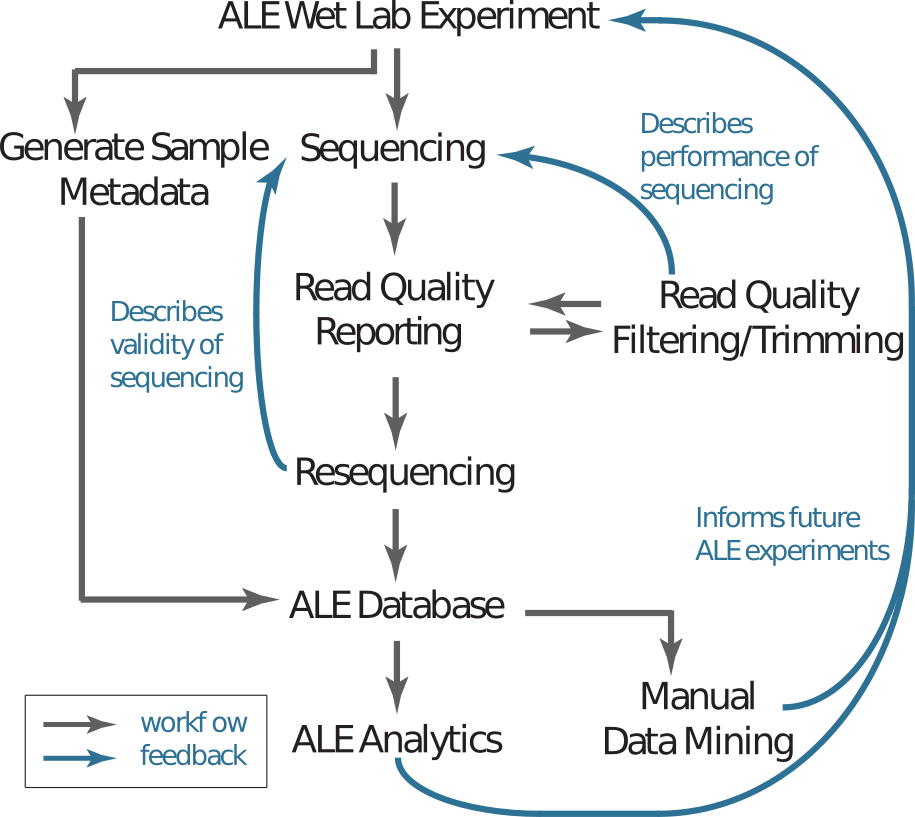
\includegraphics[width=0.7\textwidth]{post_processing_protocol.png}
  \label{fig:post_processing_protocol}
\end{figure}

We've established a post-processing protocol for the quality control of the sequencing data and to capture each sample's mutations. The protocol uses the following software: \textit{FastQC} \cite{Andrew:2010:Online} for sequenced reads quality analysis, the \textit{FASTX-Toolkit} \cite{FASTX-Toolkit} for trimming sequenced reads, and \textit{Breseq} \cite{breseq_paper} to align reads to a reference and identify mutations relative to a reference genome.

The protocol first requires that the reads for all sequenced ALE samples are inspected for their \textit{per base sequence quality} and \textit{per base sequence content} using \textit{FastQC}. The \textit{per base sequence quality} report presents the cumulative quality score of the bases in specific read positions as having good, reasonable or bad quality. From these results, we can understand which 3' and 5' read end positions have the lowest cumulative quality and trim these positions out using the \textit{FASTX-Toolkit}. We additionally inspect the \textit{per base sequence content} for any abnormalities such as the biasing for particular bases in specific positions. In a random library, you would expect that each position has approximately equal count of each base, though in our more recent samples, we often experience a biasing of base types in the first 17 positions and the final 25 positions of each read. At this point, we had additionally noticed that many alignment artifacts being identified as mutations in our subsequent variant calling were located in these read regions. This base type biasing is likely due to the sequencing library preparation chemistry that inherits an intrinsic DNA fragmentation sequence bias. Though this bias does occur, it should theoretically not result in inappropriate base calling. Even so, trimming these bias regions out of our reads has lead to less mutation calling due to sporadic non-consensus bases. The process of quality inspection and trimming may iterate multiple times before moving on. Once the reads report acceptable quality, \textit{Breseq} is used to align each sample's reads to a reference genome and identify mutations. In addition to mutations, \textit{Breseq} reports return the alignment statistics of \textit{Mean Coverage} and \textit{Mapped Read} count. In combination with the amount of unassigned missing coverage evidence, regions where no reads could be aligned to the reference, these statistics are used to evaluation the alignment performance, where we compare each statistic and \textit{unassigned missing coverage} artifact count to an empirically derived threshold. If the \textit{Mean Coverage} or \textit{Mapped Read} values fall below our thresholds or the \textit{unassigned missing coverage} artifact count exceeds our thresholds, we consider the sample they belong to as potentially problematic in our analysis of the evolution and may again sequenced the sample or discard them from the analysis.

Besides the actual generation of mutation data, the key functionality of our protocol is the stage dependent feedback provided. This feedback offers the opportunity for experimental protocol and data acquisition refinement that can be acted on by the many individuals involved in the sample sequencing pipeline.

% * <pphaneuf@eng.ucsd.edu> 2016-10-18T02:58:09.248Z:
%
% TODO: Give example of how this protocol increased our results quality and consistency.
%
% ^ <pphaneuf@eng.ucsd.edu> 2016-10-18T02:59:49.020Z:
%
% Example of results quality increase was given in an ALE Happy Hour meeting a while back, though this includes data from projects that aren't yet public.
%

\chapter{Aim 2: Automate ALE Experiment Results Consolidation and Reporting}

% * <pphaneuf@eng.ucsd.edu> 2016-10-13T18:05:59.630Z:
%
% Should I GENERALLY describe the schema of the ALE mutation database?
%
% ^.

%The products of this thesis have been primarily driven by the need to consolidate and report on large amounts of ALE experimental data in such a way to describe the quality of the sample sequencing, adaptive mutations in evolved strains, the context of mutations via their meta data (i.e., culturing environments, strain properties), and related mutations found in other experiments housed in an ALE mutation database. We have done so by leveraging a full stack of technologies that enable the parsing and databasing of experiment mutation and meta data, the execution of automated analysis on said data and the generation of web accessible reports.

% The process of accumulating all ALE experiment mutation data into a query-able uniform resource has lead us to employ current databasing technologies. The \textit{ALE mutation database} is the product of this process, containing and organizing all \textit{ALE experiment} mutations and meta data ultimately employed by the other products of this thesis.

The products of this thesis have been primarily driven by the need to consolidate and report on large amounts of ALE data in such a way to describe adaptive mutations in evolved strains. We have done so by leveraging a full stack of industry standard technologies that enable the parsing and databasing of experiment data and the generation of reports on said data.

\begin{figure}[h!]
  \caption{Illustration of the flow of ALE experiment data to the deployment of result report generation for end users.}
  \centering
  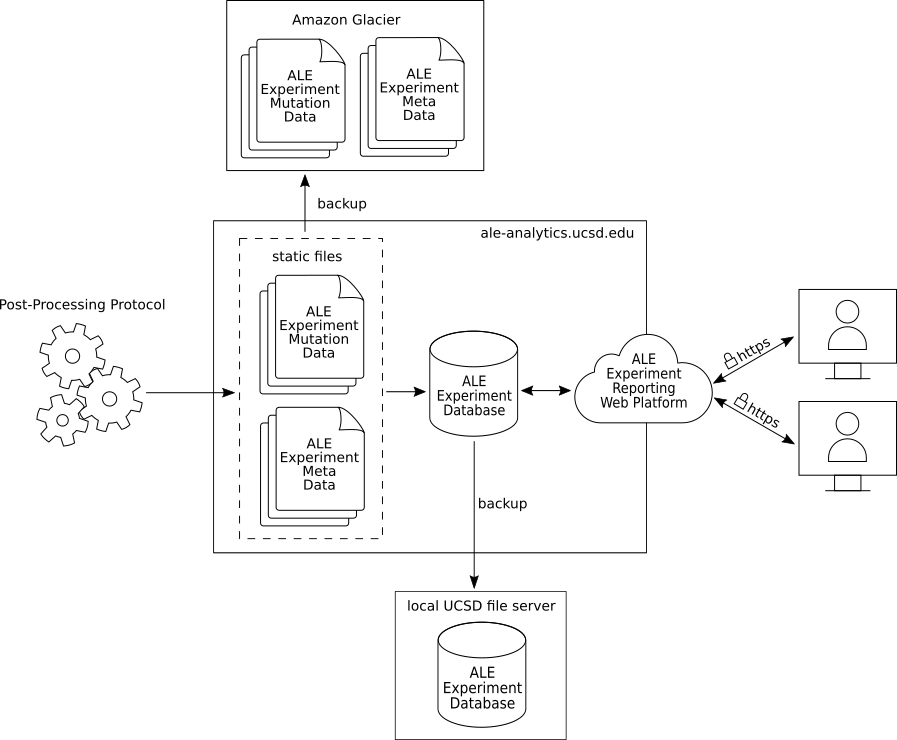
\includegraphics[width=0.7\textwidth]{deployment_diagram.png}
  \label{fig:deployment}
\end{figure}

The automation manifests as the programmatic parsing of the mutation reports generated by \textit{Breseq} for all ALE experiment samples and with the mutational data subsequently loaded into an ALE mutation database. During the initiation of an ALE experiment, experimentalists generate meta-data which can be additionally parsed and uploaded to the ALE mutation database by the automated parsing of ALE experiment data. This process consolidates all experiment mutation data and meta-data into one resources. This database is used for all ALE experiments and therefore has resulted in all available ALE experiments being consolidated into one database, enabling further cross-experiment analysis.

The ALE mutation database is leveraged by a web application to automate the generation of reports for each ALE experiment that describe the mutational lineages of their ALEs. This web application is deployed on the web, allowing for ubiquitous accessibility to ALE experiment reports for all experimentalists and collaborators. We have named this web application \textit{ALE Analytics}.

\section{ALE Analytics Web Application}

% * <pphaneuf@eng.ucsd.edu> 2016-10-21T00:48:08.332Z:
%
% Example of consistency results can be shown with the means of reporting on ALE experiment mutation results from the 4 ALE papers and how they are missing information in the papers and the full data provided in the supplementary material isn't perfect.
%
% ^.

The ALE Analytics web platform enables and automates much of the analysis necessary for interpreting ALE experiment sequencing data. For this thesis, we primarily describe the automated mutation analysis and reporting features, though this platform additionally includes ALE mutation \textit{filtering}, mutation \textit{search}, experiment \textit{export} to CSV, experiment \textit{comparison}, sample sequencing data \textit{quality statistics} and database \textit{mutation statistics}. Of these, the feature with the most effect on this thesis' primary topics is the mutation \textit{filter}, which is used to ignore mutations rationalized as inappropriate, such as alignment artifacts and ALE starting strain mutations, from all automated analysis on a specific ALE experiment.

The fundamental feature for the ALE Analytics web platform is report generation. Each ALE experiment can be described as a series of samples which contain both new mutations and mutations from their ancestors relative to a reference genome. Ordering the samples as columns from earliest to latest in an ALE, where each row describes the manifestation of a specific mutation among samples, can serve as a visualization to grant intuition on mutational trends. The occurrence of a mutation in a sample is annotated as a value between 0 and 1 within the cell of a mutation row for the sample. The annotated value represents the estimated frequency of this mutation among sample population \cite{breseq_paper}. Among the many mutations that manifest within an ALE experiment, mutation rows that describe the alleles of a gene in the ALE experiment will cluster together due to the sorting of mutations according to position on the genome. Due to the chronological sorting of the sample columns per ALE, a mutation that fixes across samples will manifest as sequence cells in a mutation row annotated for the manifestation of a mutation. These patterns are obvious to an observer and serve well to describe the mutation trends in an ALE experiment.

\begin{figure}[h!]
  \caption{Illustration of a mutation lineage report. The \textit{hns, tdk} intergenic mutation can be seen to fix over time course of samples. The multiple mutation rows describing an allele of the intergenic region \textit{ttdR, ttdA} cluster together.}
  \centering
  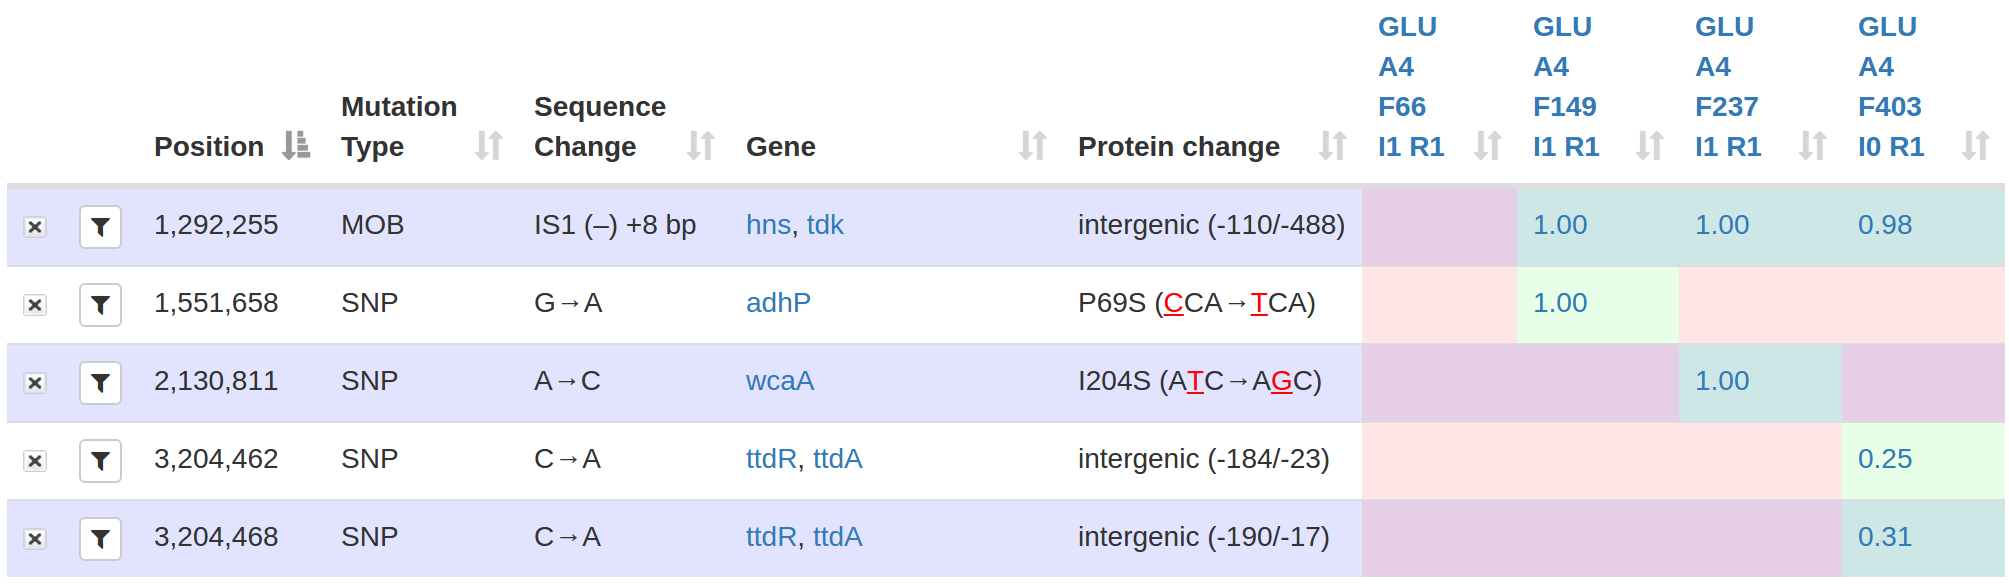
\includegraphics[width=1\textwidth]{mutation_lineage_report.png}
  \label{fig:mutation_lineage_report}
\end{figure}

% * <pphaneuf@eng.ucsd.edu> 2016-10-20T03:12:25.010Z:
%
% TODO:  ensure that the following paragraph is appropriate and shouldn't be placed elsewhere. It could be used to describe the significance of the platform, which is appropriate for this section.
%
% ^.
Before the ALE Analytics platform was deployed for use, ALE experimentalists would work to identify ALE experiment \textit{key mutations} by manually annotating all ALE experiment sample mutations within a spreadsheet and investigate for significant mutation patterns. The task of manual annotation of mutations proved to be time consuming and error-prone, causing delay of ALE experiment result interpretation. This initial bottleneck in the post-processing of ALE experiment results lead to the efforts that began the ALE Analytics project. The time cost of this manual curation additionally set an implicit limit on how many samples experimentalists were willing to sequence, therefore limiting the resolution on an ALE experiment's mutational trends. Additionally, the type of sample obtained from a flask was limited by the cost of manual curation according to the amount of mutations annotated per sample, where population samples can include an order of magnitude more mutations than clonal samples, therefore limiting the inclusion of population samples into an ALE experiment's output data set. The primary function of the ALE Analytics platform is to automate the annotation and reporting of all ALE Experiment sample mutations in a single location with a uniform format. This automated functionality enables experimentalists to more quickly interpret their data and include more sequenced samples into their mutation set, without fear of the effort necessary in consolidating their experiment's mutations. Alongside the \textit{ALE machine}, ALE Analytics further enables more resolution on evolution. This automation may additionally result in more  consistent reporting and accurate results since it removes the potential for human error in data consolidation and report generation.

Since August 2015, the ALE Analytics web application has deployed a production version for experimentalists and collaborators to use in the analysis of their ALE experiments. Though we have many development versions that are launched and shutdown for testing and demonstrating new feature to target audience, our production version of ALE Analytics has constant uptime and is available online for access by local and remote experimentalists and collaborators. To end-users, ALE Analytics represents a web platform and database of experimental evolution results that is ubiquitously available and ever growing in features and content.

\begin{figure}[h!]
  \caption{Screenshot of the ALE Analytics dashboard containing counts of significant ALE details.}
  \centering
  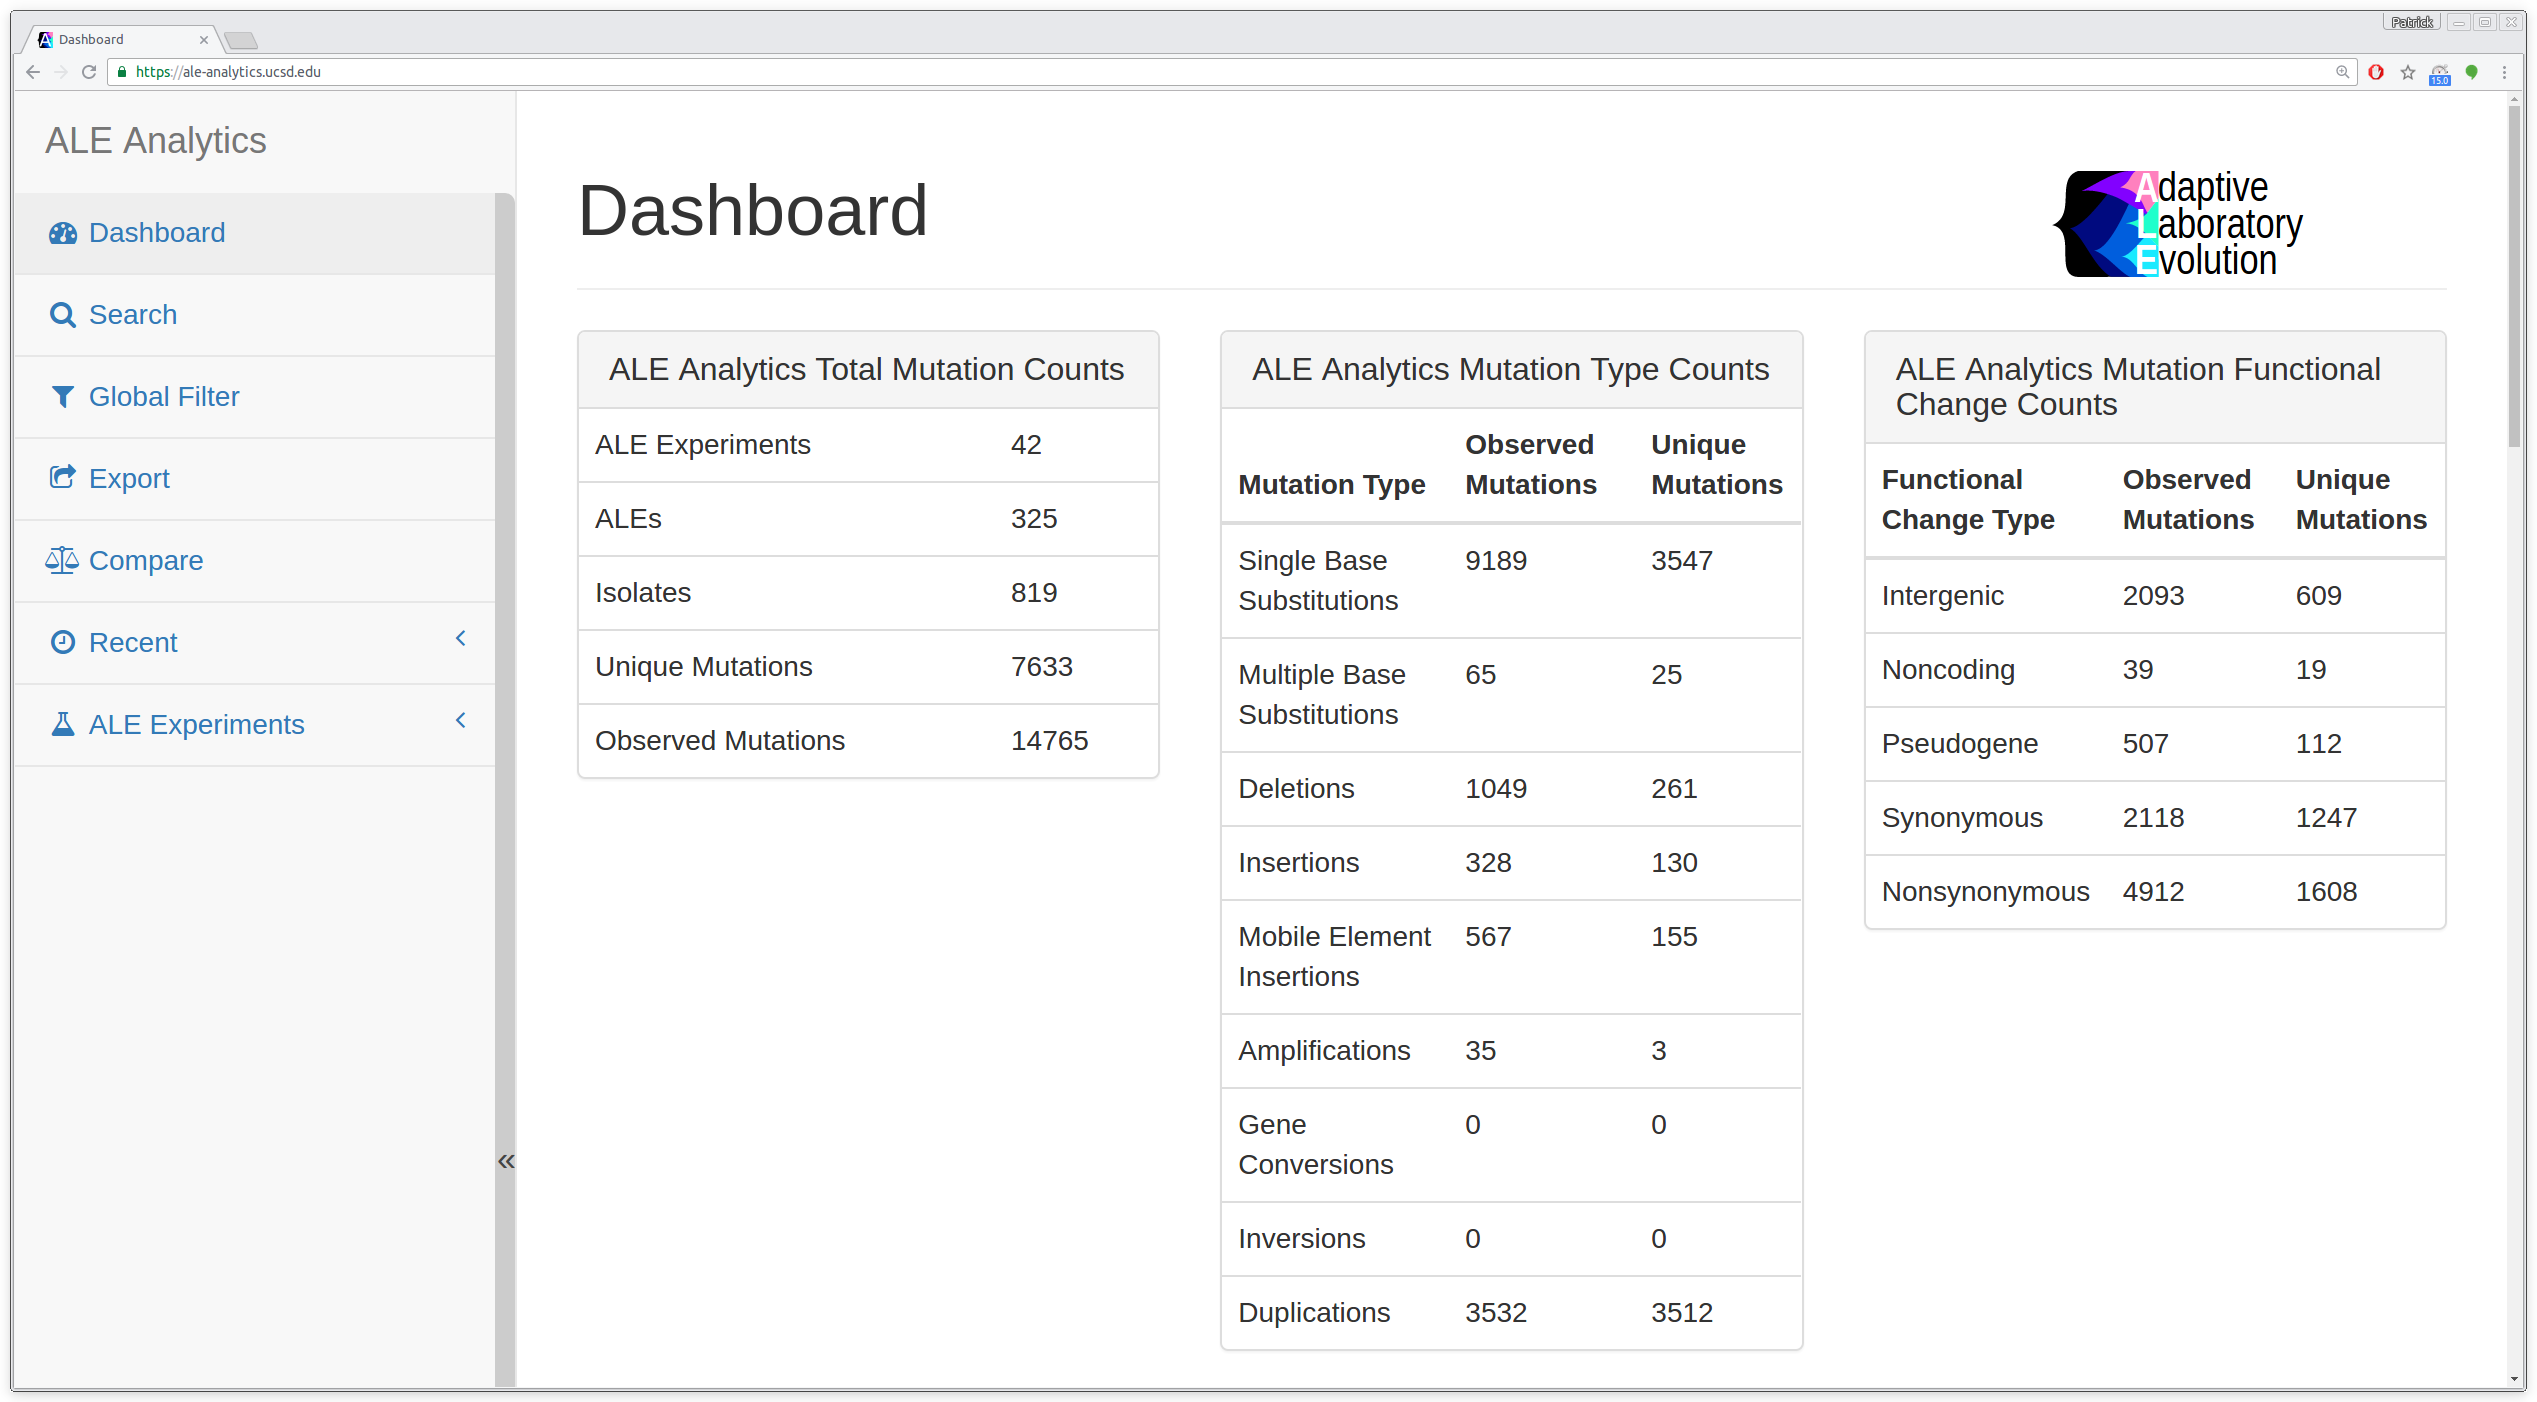
\includegraphics[width=1\textwidth]{dashboard_screenshot.png}
  \label{fig:dashboard_screenshot}
\end{figure}

The current production deployment of ALE Analytics contains 14,358 observed mutations and 7,268 unique mutations. These mutations are housed in 41 separate ALE experiments with a total of 321 ALEs and 801 isolates or samples. This large volume of mutations and samples is evidence to how the the automation of consolidating ALE experiment data has been leveraged to create a substantial resource on experimental evolutions. Being that ALE Analytics is being leveraged in investigating current experiments, full access hasn't yet been made available to the public. The set of ALE experiments with published results will be made public on ALE Analytics in the near future.

% * <pphaneuf@eng.ucsd.edu> 2016-10-20T17:06:22.581Z:
% 
% TODO: could insert figure here that describes:
% 1) more ALEs.
% 2) more samples per ALE
% 3) population samples rather than clonal samples
% 
% ^.


\chapter{Aim 3: Automate Common ALE Experiment Analysis}

Using the ALE Analytics mutation reporting mechanism, we've implemented features that find and report mutations which describe significant mutation patterns within an ALE experiment. These feature describe the significant mutation patterns as \textit{enrichment} and/or \textit{fixed} mutations. The methodologies encapsulated in the \textit{enrichment} and \textit{fixed} mutation analysis are those which have been developed to manually identify \textit{key mutations} within the results of publish ALE experiments (\cite{10.1371/journal.pgen.1001186}, \cite{pmid25015645}, \cite{pmid26964043}, \cite{pmid25304508}) and are therefore considered common ALE experiment analysis. As with the manual consolidation of ALE experiment mutations, the analysis of \textit{key mutations} can be prone to human error, inconsistent between researchers and time consuming. The automation of these common analysis will contribute to more accurate results, more consistent analysis and the shortening of turnaround time from ALE experiment execution to results interpretation.

% * <pphaneuf@eng.ucsd.edu> 2016-08-13T23:12:01.842Z:
%
% identifying mutations in the same gene/region across replicate experiments Mutation persists across many samples (fixation); Specific mutation no longer detected, but another mutation in the same gene was identified; Found at multiple points of clonal analysis -GLU paper
%
% ^.

\section{Enrichment Mutation Analysis}

% * <pphaneuf@eng.ucsd.edu> 2016-08-13T23:19:05.611Z:
%
% "These key mutations were straightforward to identify as the given genetic regions were reproducibly mutated across multiple ALE experiments." -GLU
%
% ^.

% * <pphaneuf@eng.ucsd.edu> 2016-08-14T21:56:31.904Z:
%
% "Several genes and genetic regions were identified that contained mutations across many of the independent ALE experiments, implying causality." -GLU paper
%
% ^.

% * <pphaneuf@eng.ucsd.edu> 2016-08-13T21:53:16.311Z:
%
% "This mutational recurrence pointed to the key genetic targets underlying the evolved fitness increase."
%
% ^.

Early ALE experiments only sequenced ALE endpoint samples. \textit{Key mutations} were identified as those involved in the following two cases. If a mutation manifested in more than one sample, it signified that this mutation likely rendered a fitness benefit. If a genomic region was mutated via different mutations across multiple samples, this signified that simply perturbing the gene rendered a fitness benefit. Considering that these circumstances all involve populations mutating the same genomic region, we can also consider a genomic region with multiple mutations within the same sample to possibly represent multiple populations gaining a fitness benefit by simply perturbing a genomic region. These cases can all be simplified to identifying genomic regions within an ALE experiment that have more than one observed mutation; we consider these \textit{enriched} genomic regions and their mutations as \textit{key mutations}. Previous to ALE Analytics, this analysis was accomplished as additional steps in manually curating the ALE experiment's mutation report such that mutations affecting the same genomic region would cluster together within a matrix of mutations and their samples. The \textit{Enrichment Mutation} analysis automates this approach.

\begin{figure}[H]
  \caption{\textit{Enrichment mutation} analysis flowchart}
  \centering
  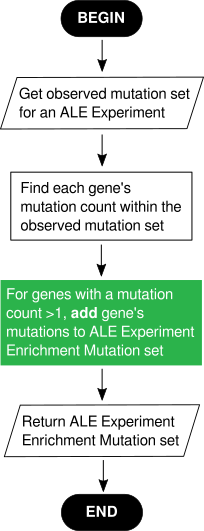
\includegraphics[width=0.3\textwidth]{enrichment_mutation_flowchart.png}
\end{figure}

\section{Fixed Mutation Analysis}

A \textit{fixed} mutation is one in which a mutation manifests in an ALEs midpoint sample and is propagated to all following samples in the lineage. \textit{Fixed mutations} are the most likely indicators of \textit{key mutations}. This analysis is possible if an ALE experiment includes midpoint samples, so as to provide for the possibility of more than one data point per mutation. Previous to ALE Analytics, the identification of \textit{fixed mutations} was accomplished as an additional curation step to results reporting by manually organizing mutations according to their sample's sequence in an ALE and and identify mutations that emerge in a midpoint and manifest in all remaining ALE samples. The \textit{Fixed Mutation} analysis automates this approach.

\begin{figure}[H]
  \caption{\textit{Fixed mutation} analysis flowchart}
  \centering
  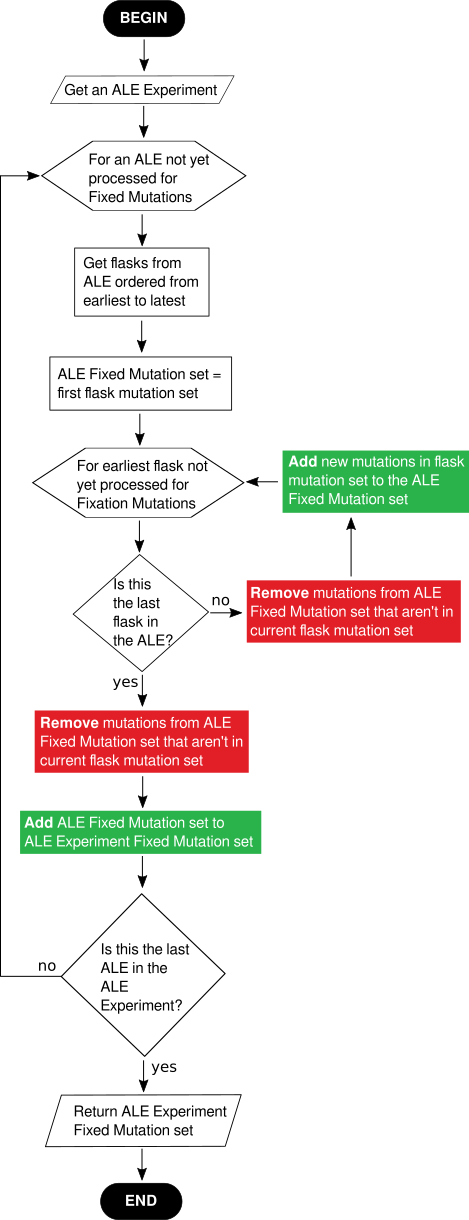
\includegraphics[width=0.50\textwidth]{fixation_mutation_flowchart.png}
\end{figure}

\begin{figure}[H]
  \caption{\textit{Ascending Frequency Fixed mutation} analysis flowchart}
  \centering
  
\includegraphics[width=0.4\textwidth]{ascending_freq_fixation_mutation_filter_flowchart.png}
\end{figure}

% * <pphaneuf@eng.ucsd.edu> 2016-10-11T02:21:34.569Z:
%
% The fixating mutation analysis additionally has a filter that enables this analysis to remove all fixation mutations which include a population sample based mutation that descends in frequency relative to the previous ALE sample. This feature is referred to as the Ascending Frequency Filter. This filter has been implemented to remove any mutations that seemingly fixate though show sporadic frequencies and therefore shouldn't be considered primary beneficial mutations. For GLU, no fixation mutations were removed when applying this filter after removing fixations due to hypermutators.
%
% ^.

% * <pphaneuf@eng.ucsd.edu> 2016-10-14T16:43:26.019Z:
%
% TODO: Include description of Ascending Fixed Mutations filter
%
% ^.
\section{Results}

% * <pphaneuf@eng.ucsd.edu> 2016-10-11T02:35:45.973Z:
%
% TODO: We also investigate any new key mutations by ALE Analytics and potentially corroborate these new findings with the published materials.
%
% ^.

To ensure that our automated \textit{key mutation} analysis returns \textit{key mutations} based on published criteria, we evaluate it's the automated analysis results against those found in ALE experiments published by UCSD's Systems Biology Research Group. The automated analysis \textit{key mutations} are generated by incorporating the sample reads available from these published ALE experiments into the post-processing protocol, ALE Analytics platform and \textit{key mutation} automated analysis. Intuitively, our task can be described as finding all of the \textit{key mutations} within the complete set of mutations in an ALE experiment and comparing the set for equality against the published \textit{key mutation} set of the same experiment. The post-processing protocol will be configured to reproduce as well as possible the mutation set used by the authors of the publish materials by using the same reference genome and \textit{Breseq} version. This does not guarantee that the mutation set produced will be identical to those used by the authors and therefore introduces the issue of having different starting conditions between \textit{key mutation} analysis.

% * <pphaneuf@eng.ucsd.edu> 2016-10-22T17:45:47.614Z:
%
% Talk towards what are the probabilistic circumstances that cause the potential for different mutations to be called from those used in the papers to identify key mutations.
%
% ^.

We therefore shouldn't simply compare the \textit{key mutation} output of the different methods but rather find a more practical comparison. Clarification of gene function is a primary result in ALE experiments. Organisms studied in ALE experiments are selected for their phenotype which is derived from their genotype. The areas of the genotype of highest interest as those genomic regions perturbed by mutations. With the ALE experiment mutation set, experimentalists investigate the known function of the perturbed genomic region, the result of the mutation's perturbation and infer any additional function of the genomic region. We can therefore reason that a better evaluation between the results of the published ALE experiments and the ALE Analytics automated analysis is a comparison of the genomic regions found to be perturbed by \textit{key mutations}. We discuss any false positives and false negatives and determine why they manifest and what can be implemented to handle their specific cases. The following is a set of publications that we use in our evaluation and their ALE Experiment names:
\begin{itemize}
\item \textbf{The PGI ALE Experiment}: \textit{Genetic Basis of Growth Adaptation of Escherichia coli after Deletion of pgi, a Major Metabolic Gene.} \cite{10.1371/journal.pgen.1001186}
\item \textbf{The 42C ALE Experiment}: \textit{Evolution of Escherichia coli to 42 °C and Subsequent Genetic Engineering Reveals Adaptive Mechanisms and Novel Mutations. Molecular Biology and Evolution.} \cite{pmid25015645}
\item \textbf{The 13C ALE Experiment}: \textit{Evolution of E. coli on [U-13C]Glucose Reveals a Negligible Isotopic Influence on Metabolism and Physiology.} \cite{pmid26964043}
\item \textbf{The GLU ALE Experiment}: \textit{Use of Adaptive Laboratory Evolution To Discover Key Mutations Enabling Rapid Growth of Escherichia coli K-12 MG1655 on Glucose Minimal Medium.} \cite{pmid25304508}
\end{itemize}
\section{Evaluation}
In this section we describe our approach to formally evaluating the performance of our \textit{key mutation} automate analysis. The task of finding \textit{key mutations} is a binary classification problem, where a mutation is or is not \textit{key}. To accomplish binary classification on a set of mutations, we've defined a set of features that describe how a mutation should be classified: the \textit{enrichment} mutation feature and the \textit{fixed} mutation feature. If a mutation qualifies for either feature, we will classify this mutation as a \textit{key mutation}.

In establishing our classification evaluation metrics, we observe that there are many more \textit{insignificant} mutations than \textit{key mutations} mutations, or in other words, there exists a class imbalance.

\begin{figure}[H]
  \caption{\textit{Key mutation} and \textit{insignificant} mutation class imbalance. The \textit{key mutation} count is obtained from the ALE experiment published materials and the \textit{insignificant} mutation count is obtained by finding the difference between the \textit{key mutation} count and the total mutation count from our variant finding results of an ALE experiment. We use our variant finding total mutation count for consistency since some published ALE experiments didn't include the total set of observed mutations in their supplementary material}
  \centering
  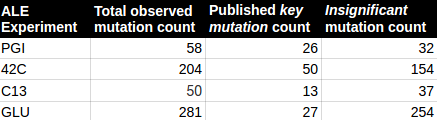
\includegraphics[width=0.6\textwidth]{class_imbalance_table.png}
  \label{fig:class_imbalance_table}
\end{figure}

We demonstrate this imbalance in Figure\ref{fig:class_imbalance_table}. All but the \textit{PGI ALE experiment} have an obvious class imbalance. Relying on accuracy alone to measure classification performance with a class imbalance can be misleading since one could naively classify all mutations as the majority class of the imbalance and still obtain a high accuracy. We consider avoiding the exclusion of \textit{significant} mutations from our results as our highest priority; in other words, we consider \textit{recall} as our primary performance metric. In performing with high \textit{recall}, we can better ensure that all \textit{key mutations} are returned in our results, therefore providing the best identification of all significant genomic regions in an experimental evolution. Avoiding \textit{insignificant mutations} in our results is of secondary importance since they can be later excluded by secondary manual investigations performed by the experimentalist. We will use \textit{precision} as the metric to evaluate our approach's ability to avoid \textit{insignificant} mutations in our results.

\subsubsection{PGI ALE Experiment}
% * <pphaneuf@eng.ucsd.edu> 2016-08-13T20:14:33.404Z:
%
% "The gene \textit{pgi} catalyzes the isomerization of glucose 6-phosphate to fructose 6-phosphate in upper glycolysis. Removal of this gene forces the glycolytic flux through the pentose phosphate pathway, creating a redox imbalance due to excess NADPH production ."
%
% ^.
The \textit{PGI ALE experiment} and publication focused on the observed adaptive mutations selected for during an experimental evolution due to the knocking out the phosphoglucose isomerase \textit{pgi} gene from the K-12 strain of \textit{E. coli}. The \textit{pgi} gene plays a major role in the central metabolism of E. coli and is a good candidate for studying how a strain learns to compensate for a loss of such significant impact. The experiment executed 10 parallel ALEs on replicates of \textit{E. coli K-12 MG1655} lacking the \textit{pgi} gene using ALE methodologies for 50 days in minimal media. Clones were taken from each ALE's final flask and their mutations were defined by first whole-genome sequencing through both Nimblegen hybridization-base tiling arrays and Illumina Solexa technologies, then leveraging the Nimblegen's built-in variant calling capabilities and in-house software. PCR and Sanger sequencing was additionally used to verify mutations identified and the entire sequence of host genomic regions \cite{10.1371/journal.pgen.1001186}. Our analysis of the \textit{PGI ALE experiment} samples was executed by processing the same reads generated by the authors using the \textit{Breseq} 0.23 software pipeline against the \textit{E. coli K-12 MG1655} reference genome (NCBI accession NC\_000913.2).
% * <pphaneuf@eng.ucsd.edu> 2016-09-22T00:24:29.708Z:
%
% Why was PGI 9 not included in the paper?
%
% ^ <pphaneuf@eng.ucsd.edu> 2016-09-22T03:16:46.041Z:
%
% Adam has responded with the idea that they believed something was poor about their resequencing and therefore they didn't included it in the analysis. Not a problem for this thesis since no significant mutation analysis used PGI 9 data.
%
% ^ <pphaneuf@eng.ucsd.edu> 2016-09-22T16:53:17.283Z.

\begin{figure}[H]
  \caption{\textit{PGI} ALE experiment \textit{key mutation} genomic region matching summary between the paper and the ALE Analytics automated \textit{enrichment key mutation} analysis}
  \centering
  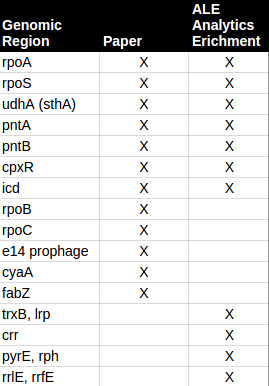
\includegraphics[width=0.4\textwidth]{pgi_key_mutation_regions.png}
    \label{fig:pgi_key_mutation_regions}
\end{figure}
The \textit{PGI} ALE experiment paper doesn't explicitly list the \textit{key mutations} as does the other ALE experiment papers involved in our evaluation. We therefore rationalize the paper's \textit{key mutations} according to the findings presented on each mutation and their host genomic region. The \textit{PGI} experiment publication identified the perturbation of the following genes as being important for the experiment's observed fitness:

\begin{itemize}
\item \textit{rpoS}: mutations observed suppresses stress response by modulating transcription; likely fitness selection in relation to the adaptation to loss of \textit{pgi}.
\item \textit{rpoA}, \textit{rpoB}, \textit{rpoC}, \textit{cpxR} and \textit{cyaA}: mutations observed result in global network-level transcriptional regulation adaptions.
\item \textit{sthA}, \textit{pntA}, \textit{pntB}: mutations observed counters the redox imbalance of excess NADPH production due to \textit{pgi} knockout.
\item \textit{e14 prophage deletion}: target and mutations observed are mechanistically unknown, yet experimental data shown to provide fitness.
\end{itemize}

The authors speculate that the deletion of the \textit{e14 prophage} is a unique contributor to the fitness of the host strain since they were not able to reproduce its attributed fitness with any combination of other \textit{key mutations} in followup ALEs. The \textit{e14 prophage} deletion manifests as unassigned missing coverage in our variant reports, to which we include in our ALE Analytics database but currently do not yet include in reports. The authors do mention the potential importance of the \textit{icd} SNPs resulting correlated with this deletion. It is speculated that these SNPs may have a fitness benefit in their potential to induce better translation efficiency to \textit{icd}. Due to the high frequency of these \textit{icd} SNPs, the \textit{enrichment} analysis did include them in its results as \textit{key mutation}. Though no solid evidence could be found on the \textit{icd} allele's fitness benefit, since the authors speculate that the \textit{icd} mutations are significant and the objective of the ALE Analytics automated analysis is to highlight the mutation that may be a result of the ALE's selective pressures, we consider the paper's \textit{icd} SNPs to be \textit{key mutations}.

Of the 12 \textit{key mutations} alleles published in the paper, the \textit{enrichment} analysis is successful in finding 7. The ALE Analytics \textit{enrichment} analysis finds multiple \textit{icd} alleles in both ALE 1 and ALE 5. \textit{icd} alleles were reported to be associated with the \textit{e14 prophage } deletion, published as occurring in the ALE 1. The evidence of high \textit{icd} enrichment in ALE 5 motivated an investigation into the possibility of an ALE 5 \textit{e14 prophage} deletion that was in fact found. This investigation serves to elaborate on the importance of automating \textit{key mutation} identification for ALE experiments.

A minority of the published \textit{key mutations} which didn't manifest more than once were included in the paper's \textit{key mutation} set according to their functional association with significantly enriched genes. SNPs uniquely affecting transcription modulation genes \textit{cyaA}, \textit{rpoB}, and \textit{rpoC} were included as \textit{key mutations} in the paper in addition to the mutations of the more frequently mutated \textit{rpoA}, \textit{rpoS} and \textit{cpxR} genes. These \textit{key mutations} could be included in future \textit{enrichment} analysis implementations by additionally considering the mutational \textit{enrichment} of functional groups rather than only single genes.

The \textit{fabZ} SNP was speculated as important by the authors due to their knowledge of the potential metabolic perturbations caused by the \textit{pgi} knockout and the idea that the this mutation may reduce it's impact. This type of \textit{key mutation} could be included in future \textit{enrichment} analysis by including functional data on any type of perturbation introduced into the initial strain of the experimental evolution and identify mutations affecting genes associated with functionality related to the initial perturbation. This approach would therefore also leverage the enrichment of functional groups of genes.

Published mutations in the \textit{rep}, \textit{yfeH}, \textit{fruK}, \textit{rodA}, \textit{bipA} and \textit{ispU} genes only manifest once and weren't discussed by the publication as being \textit{key mutation}. These mutations were therefore not considered for either the publication's \textit{significant} mutation set and the ALE Analytics \textit{enrichment} analysis evaluation.

The ALE Analytics \textit{enrichment} mutation analysis found 4 additional possible \textit{significant} genomic regions described in Figure \ref{fig:pgi_new_enrichment_muts} due to their frequency of mutation. Though these new \textit{enriched} genomic regions contributed to the lessening of the \textit{enrichment} analysis' precision metric, they present an opportunity for identifying further \textit{significant} adaptions not caught by the authors.
\begin{figure}[H]
  \caption{New \textit{PGI} ALE experiment \textit{enrichment key mutations}. The value \textit{1} used to denote the presence of a mutation describes the approximate frequency in which the mutation was found within the sample population represented in the sample reads \cite{breseq_paper}}.
  \centering
  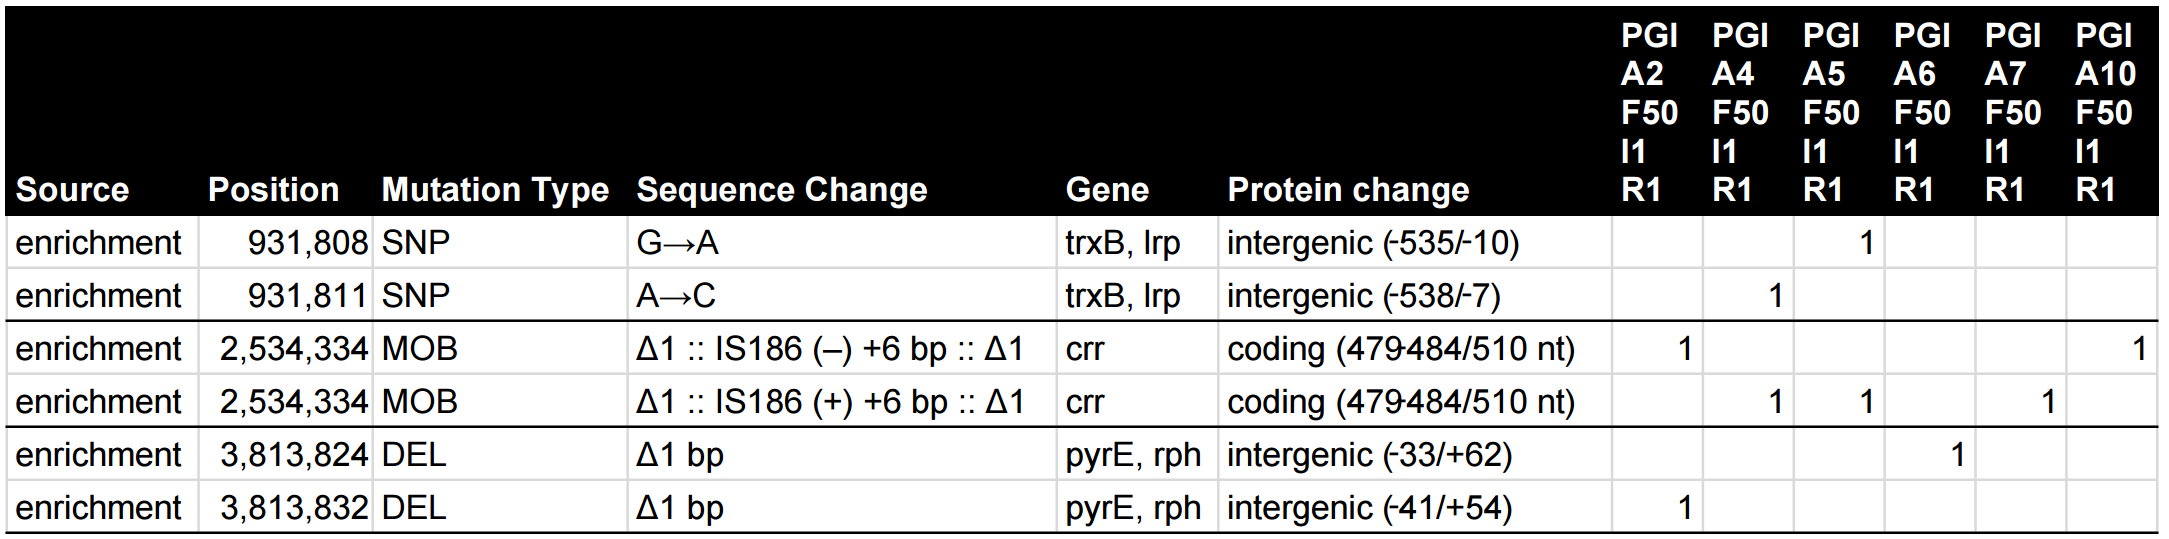
\includegraphics[width=\textwidth]{pgi_new_enrichment_muts.png}
  \label{fig:pgi_new_enrichment_muts}
\end{figure}
\begin{figure}[H]
  \centering
  \caption{\textit{PGI} ALE experiment classification results.}
  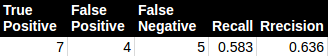
\includegraphics[width=0.6\textwidth]{pgi_precision_recall.png}
\end{figure}

No fixed mutations can be established with the \textit{PGI} ALE experiment data set since all samples are endpoints of different ALEs and therefore do not provide any mutation time-course information for the \textit{fixed} mutation analysis to work with.
\subsubsection{42C ALE Experiment}
The \textit{42C} ALE experiment and publication focused on the observed adaptive mutations selected for during an experimental evolution with a selective pressure of a sample temperature of 42$^{\circ}$C. The experiment executed 10 parallel ALEs on replicates of \textit{E. coli K-12 MG1655} for 45 days in minimal media. Clones were taken from each ALE's final flask, sequenced using the Illumina MiSeq platform and their mutations defined using whole genome re-sequencing with the \textit{Breseq} 0.22 software pipeline against the \textit{E. coli K-12 MG1655} reference genome (NCBI accession NC\_000913.2) \cite{pmid25015645}.

The authors of the \textit{42C} paper considered \textit{key mutations} as those that perturbed a gene in more than one ALE endpoint. Their \textit{key mutation} results were clearly annotated in a Table 2 \cite{pmid25015645}. This ALE experiment experience the manifestation of two different hypermutator strains, proposed as independently manifesting in ALE 2, where \textit{mutL} was mutated, and ALE 6, where \textit{dnaQ} was mutated. The ALE 2 hypermutator strain went on to contaminate ALE 3 and the hypermutator strain in ALE 6 went on to contaminate ALE 8. Due to this contamination, the authors didn't consider mutations recurring between ALE endpoints derived from the same hypermutator strain as \textit{key mutations}. The authors did observe unique mutations occurring within the same genomic region within and between hypermutator strain pairs and therefore did not completely disregard the hypermutator samples.
\begin{figure}[H]
  \caption{\textit{42C} ALE experiment {key mutation} genomic region matching summary between the paper and the ALE Analytics automated {enrichment key mutation} analysis.}
  \centering
  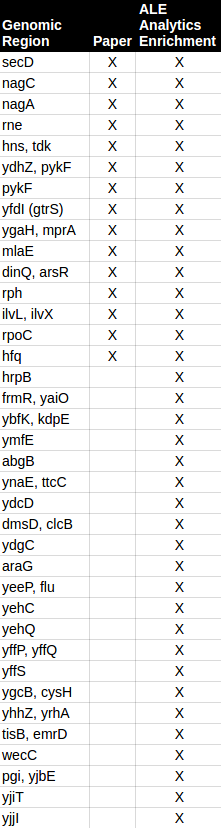
\includegraphics[width=0.3\textwidth]{42c_key_mutation_regions.png}
  \label{fig:42c_key_mutation_regions}
\end{figure}
The ALE Analytics \textit{enrichment key mutation} analysis finds all 14 of the genomic regions affected by the published \textit{key mutations}. The success of the ALE Analytics \textit{enrichment} analysis is based on the fact that its implementation stems from the protocol for identifying significant mutations in an experimental evolution established by this paper.

\begin{figure}[H]
  \caption{new \textit{enrichment key mutations}. ALE endpoint pair (2, 3) and (6, 8) are each derived from the same hypermutator strain, therefore explaining the large amount of mutations shared between the endpoints. The value of \textit{1} used to denote the presence of a mutation describes the approximate frequency in which the mutation was found within the sample population represented in the sample reads \cite{breseq_paper}}
  \centering
  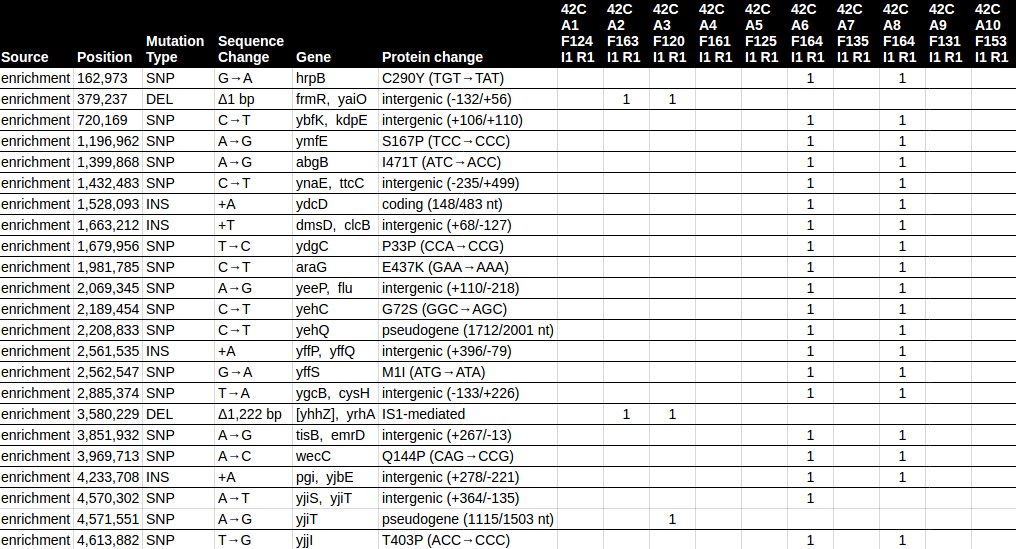
\includegraphics[width=\textwidth]{42c_new_enrich_muts.png}
  \label{fig:42c_new_enrich_muts}
\end{figure}

The ALE Analytics \textit{enrichment} mutation analysis finds 22 additional genomic regions affected by more than 1 mutation. The \textit{mutL} and \textit{dnaA} mutations mentioned by the paper as the cause for ALE 2, 3, 6 and 8 endpoints to become hypermutators were included in the automated analysis' \textit{enrichment key mutations}. The paper does not include these in their table of \textit{key mutations}, though do attribute describe their importance; we therefore do not consider the \textit{mutL} and \textit{dnaA} mutations as false positives.

\begin{figure}[H]
  \centering
   \caption{\textit{42C} ALE experiment classification results.}
  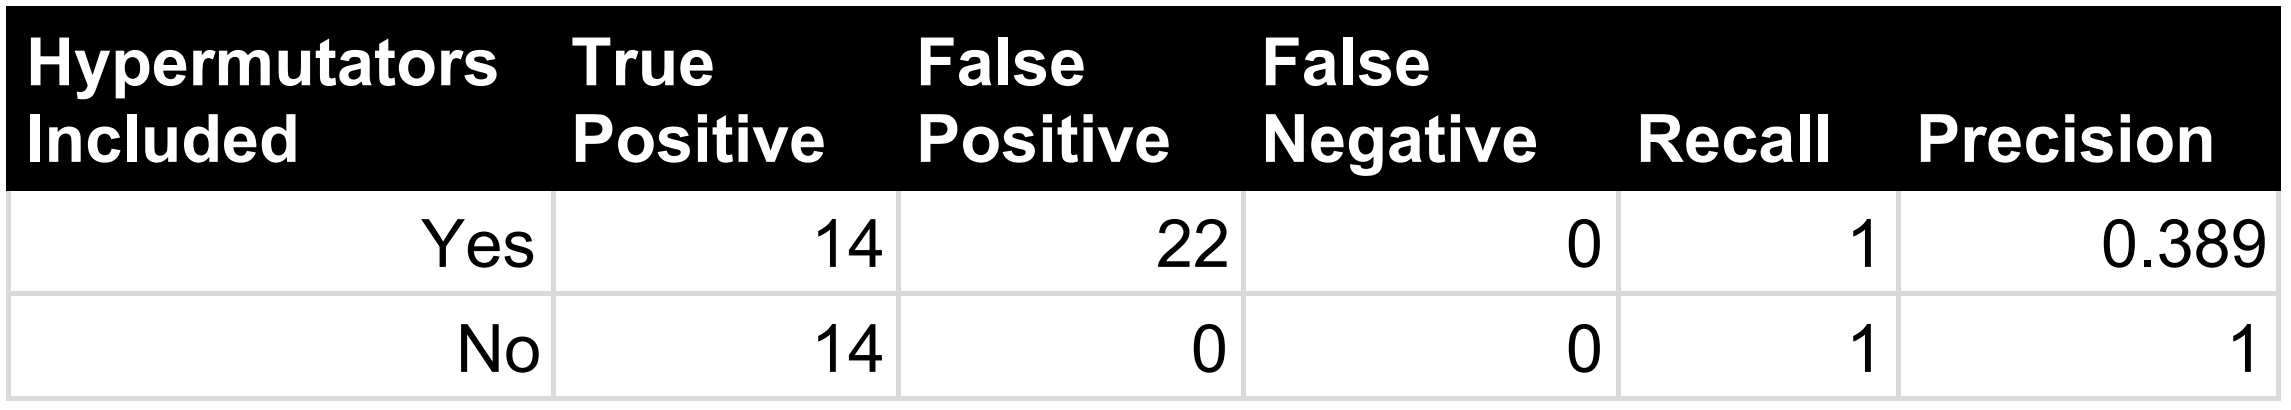
\includegraphics[width=0.5\textwidth]{42c_precision_recall.png}
\end{figure}

These 22 additional genomic regions of interest only manifest in the ALEs that have been identified by the authors as being overcome by the same hypermutator strain except for the \textit{yjiT} alleles. \textit{yjiT} was mutated in the ALE 3 and 6 endpoints, hypermutators of separate origins, and therefore make it a candidate for an appropriate \textit{key mutation}. If the exclusion of the \textit{yjiT} mutations in the author's \textit{key mutation} set may have been an oversight in their manual workflow; the automated \textit{enrichment key mutation} analysis will reduce the possibility for these errors with its future usage. If our evaluation were to exclude hypermutator mutations from both the published significant mutations list and our results, both the subsets of the non-hypermutator published and automated analysis \textit{key mutations} would match without any additionally \textit{key mutations} mutations. 

The obvious contamination made clear by the amount of hypermutator mutations in contaminated strains lends us intuition on how to automate the identification of contamination among samples. When a sample contains the exact same \textit{point mutations} as a sample from another ALE, contamination has likely occurred.

No fixed mutations can be established with the \textit{42C} ALE experiment data set since all samples are endpoints of different ALEs and therefore do not provide any mutation time-course information for the \textit{fixed} mutation analysis to work with.
\subsubsection{C13 ALE Experiment}
The C13 ALE experiment and publication focused on the observed adaptive mutations selected for during an experimental evolution using \textsuperscript{13}C-glucose as a carbon source for \textit{E. coli} growth. The \textit{key mutations} found by this experiment were compared to those of \cite{pmid25304508}, which uses \textsuperscript{12}C-glucose, to investigate if there is any evidence of differing adaptations and therefore additional metabolic stress from using the \textsuperscript{13}C-glucose isotope. The experiment executed 6 parallel ALEs  on replicates of \textit{E. coli K-12 MG1655} for approximately 1000 generations per ALE. Two clonal samples were taken from each ALE; one sample served as a midpoint clone and the other as the endpoint clone. The clones were sequenced using the Illumina MiSeq platform and their mutations defined using whole genome re-sequencing with the \textit{Breseq} 0.23 software pipeline against the \textit{E. coli K-12 MG1655} reference genome (NCBI accession NC\_000913.2).

The authors of the C13 published material considered the mutations for genes that were enriched in more than one endpoint to be \textit{key mutations}. Their \textit{key mutation} results were clearly stated as those mutations which affected the \textit{pyrE/rph}, \textit{rpoB}, \textit{hns/tdk} and \textit{rhsE} genomic regions. The ALE Analytics \textit{enrichment key mutation} analysis finds all 4 of the published genomic regions affected by \textit{key mutations}.
\begin{figure}[H]
  \caption{New \textit{C13} ALE experiment \textit{enrichment key mutations}. The value of \textit{1} used to denote the presence of a mutation describes the approximate frequency in which the mutation was found within the sample population represented in the sample reads \cite{breseq_paper}}
  \centering
  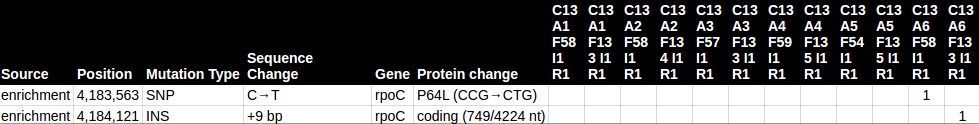
\includegraphics[width=\textwidth]{c13_new_enrich_muts.png}
  \label{fig:c13_new_enrich_muts}
\end{figure}
The ALE Analytics \textit{enrichment} mutation analysis found 1 additional possible \textit{significantly} enriched allele described in Figure \ref{fig:c13_new_enrich_muts}: \textit{rpoC}. The authors did not include \textit{rpoC} as a \textit{key mutation} since their approach was limited to high frequency alleles among different ALEs. The ALE Analytics \textit{enrichment} analysis additionally returns mutations found to affect genomic regions within multiple samples within the same ALE.

The ALE Analytics \textit{fixed key mutation} analysis finds 2 of the 4 published \textit{key mutations} alleles. Those \textit{key mutations} missed were due to only manifesting in endpoint samples taken for the ALE experiment. If the C13 ALE experiment had more midpoint samples, the fixing of these mutations may be more evident and would ultimately be captured by the \textit{fixed key mutation} analysis. Significant mutations should ultimately be all caught by the \textit{fixed key mutation} analysis with enough samples, though the question that remains is how many samples from an ALE are adequate to provide enough resolution on mutation lineages to capture all fixing mutations.
%\todo{(Could speak towards incorporating fitness growth data in future iterations to appropriately understand the necessary sample resolution for capturing sufficient mutation lineage information for fixations.)}

\begin{figure}[H]
  \caption{\textit{C13} ALE experiment {key mutation} genomic region matching summary between the paper and the ALE Analytics automated {enrichment} and \textit{fixed key mutation} analysis.}
  \centering
  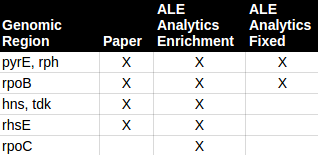
\includegraphics[width=0.4\textwidth]{c13_key_mutation_regions.png}
  \label{fig:}
\end{figure}

\begin{figure}[H]
  \centering
   \caption{\textit{C13} ALE experiment classification results.}
  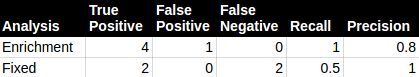
\includegraphics[width=0.5\textwidth]{c13_precision_recall.png}
\end{figure}
\subsubsection{GLU ALE Experiment}
% * <pphaneuf@eng.ucsd.edu> 2016-10-23T04:30:15.025Z:
%
% NOTE: Adam had mentioned that ALE 5 was contaminated, though it was still used in the paper for identifying key mutations. Will therefore keep it in my analysis also.
%
% ^.
The GLU ALE experiment and publication focused on establishing and leveraging novel ALE methods and observing the adaptive mutations selected for using these ALE methods and \textit{E. coli} on glucose minimal media at 37$^{\circ}$C. This experiment isolated the selection pressure to the growth rate of the strain by propagating batch cultures to new flasks during their exponential growth phase rather than the stationary growth phase; this avoids the fixation of mutations that grant fitness to attributes other than growth rates. The experiment executed 8 parallel ALEs on replicates of \textit{E. coli K-12 MG1655}, capturing samples from both the final and intermediate ALE flasks for whole genome sequencing with the Illumina MiSeq platform and re-sequencing using the \textit{Breseq} 0.23 software pipeline against the \textit{E. coli K-12 MG1655} reference genome (NCBI accession NC\_000913.2).

The authors employed two strategies for identifying \textit{key mutations}. The first was to find genomic regions that were mutated in multiple ALEs and the second was to find genomic regions that hosted multiple mutations within the same ALE. The ALE Analytics \textit{enrichment key mutation} analysis finds all 8 of the genomic regions affected by the published \textit{key mutations}.

The ALE Analytics \textit{enrichment} mutation analysis found 15 additional possible \textit{significant} genomic regions described in \ref{fig:GLU_new_enrich_muts} due to their allele frequency. Though these new \textit{enriched} genomic regions contributed to the lessening of the \textit{enrichment} analysis' precision metric, they present an opportunity for identifying further \textit{significant} adaptions not caught by the authors.

\begin{table}[h!]
\centering
\begin{tabular}{ l r }
  \textbf{recall} & 1 \\
  \textbf{precision} & 0.347826087 \\
\end{tabular}
\end{table}

\begin{figure}[h!]
  \caption{new \textit{fixation} mutations.}
  \centering
  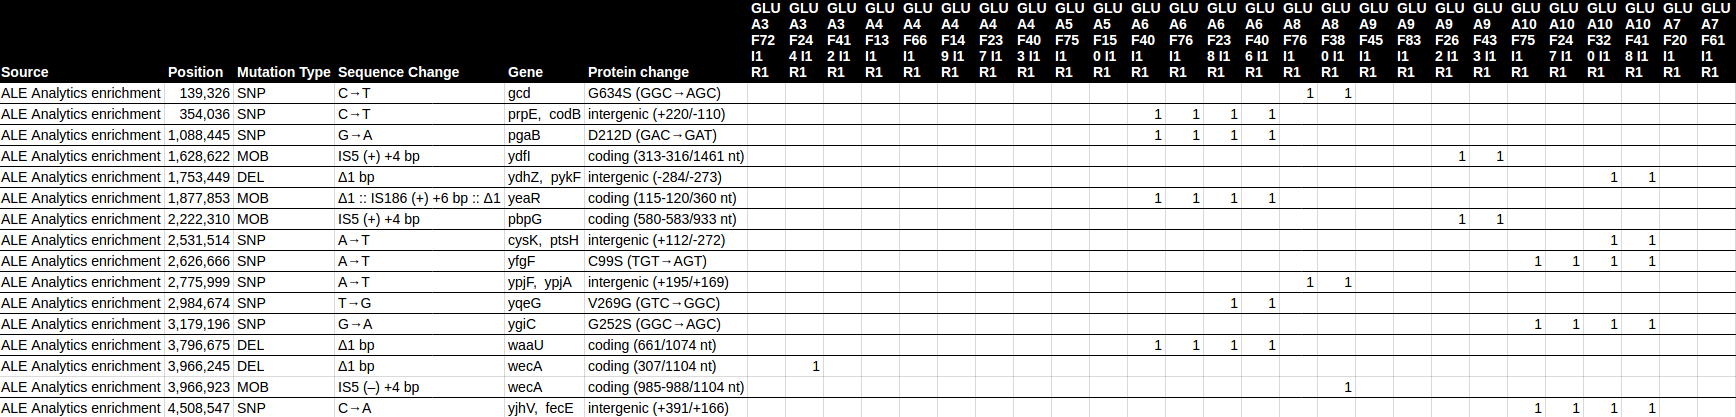
\includegraphics[width=\textwidth]{GLU_new_enrich_muts.png}
  \label{fig:GLU_new_enrich_muts}
\end{figure}

The ALE Analytics \textit{fixation} finds 14 unpublished \textit{fixed key mutations}. These \textit{fixed} mutations are the same as the set of unpublished \textit{enrichment} alleles found with the \textit{enrichment} analysis with the exception of \textit{wecA}.

\begin{table}[h!]
\centering
\begin{tabular}{ l r }
  \textbf{recall} & 0.875 \\
  \textbf{precision} & 0.3333333333 \\
\end{tabular}
\end{table}

\chapter{Aim 4: Enable More Accessible ALE Experiment Results}
\section{}
Potential for a subset of ALE experiment results to be released or accessible as a public resource.

\chapter{Discussion}

% * <pphaneuf@eng.ucsd.edu> 2016-10-11T04:04:04.439Z:
%
% the Fixating Mutations analysis is more likely to find fitness causal mutations due to it's filtering for mutations that have been obviously selected for.
%
% ^.

% * <pphaneuf@eng.ucsd.edu> 2016-08-13T23:22:12.398Z:
%
% "A persistent challenge and goal in ALE experiments is differentiating between causal mutations and genetic hitch-hikers. 57% (30 of 53) of all mutations persisted in every subsequent clone examined until the experiment ended (mutations only observed in the last clone examined for each experiment were not considered)." -GLU 
%
% ^ <pphaneuf@eng.ucsd.edu> 2016-08-13T23:22:45.381Z:
%
% This is why we need more than 1 method of identifying key mutations.
%
% ^.

% * <pphaneuf@eng.ucsd.edu> 2016-10-11T02:20:54.338Z:
%
% The fixating mutations analysis possibly returns a more refined list of key mutations due to its design of focusing on a particular mutational pattern, though this analysis can't differentiate between fixating mutations selected for their fitness benefits and hitchhiking mutations.
%
% ^.

% * <pphaneuf@eng.ucsd.edu> 2016-10-18T21:50:21.977Z:
%
% Target: ALE Mutation Database, Inputs: ALE experiment mutations, ALE experiment metadata, ALE experiment duplications.
%
% ^.

A significant result of the consolidation of ALE experiment results and reporting is that one can easily compare the results of multiple ALE experiments and search for mutational trends among all ALE experiments.

\section{Shared Enrichment and Fixated Mutations}
% We investigate if ALE Analytics features are able to find novel perspectives on the \textit{key mutations} by leveraging the the fact that all ALE experiments are unified within one database and investigate if ALE experiments share any \textit{key mutations}. 
Shared \textit{enrichment} and \textit{fixating} leverages the nature of the ALE Analytics platform to automate the identifying of genomic regions shared across all ALE Experiments that contain \textit{enriched} or \textit{fixating} alleles. In this section, we present the shared \textit{enrichment} and \textit{fixating} alleles and their mutations and elaborate on their significance.

% * <pphaneuf@eng.ucsd.edu> 2016-10-11T16:26:33.158Z:
%
% Also speak towards the metadata comparison possible.
%
% ^.

The PGI ALE experiment shared one significantly enriched genomic region with the other ALE experiments of this dataset: the \textit{rph} gene and it's upstream intergenic region with \textit{pyrE}. The \textit{rph} \textit{enrichment} alleles were shared among all of the ALE Experiments within this dataset: \textit{PGI}, \textit{C13}, \textit{42C} and \textit{GLU}. 

\begin{figure}[h!]
  \caption{Shared \textit{rph} \textit{enrichment} mutations.}
  \centering
  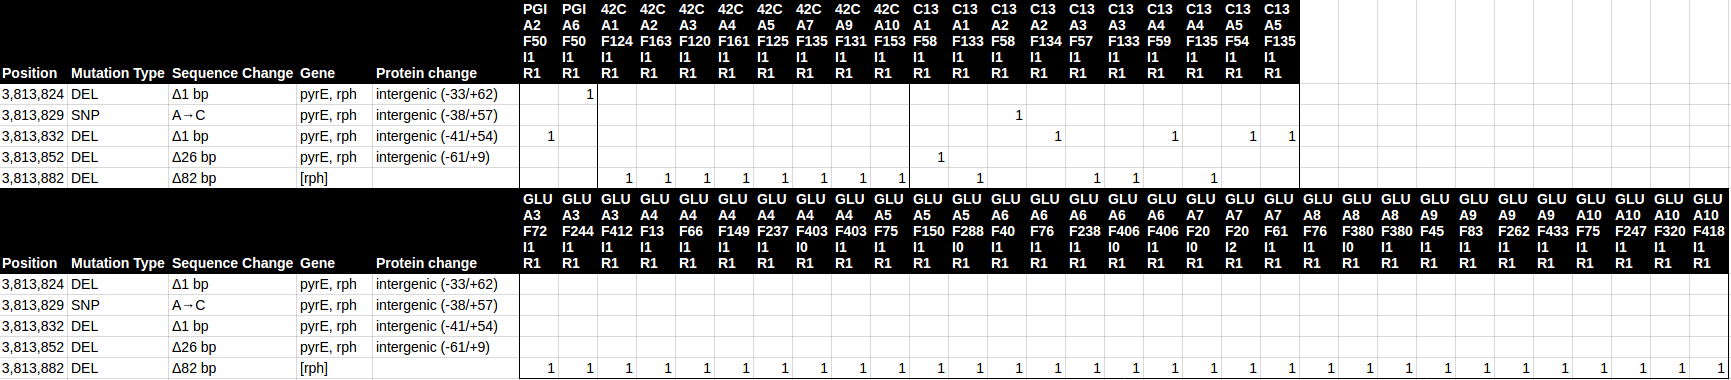
\includegraphics[width=\textwidth]{rph_pyrE_shared_enrich_mut.png}
  \label{fig:rph_pyrE_shared_enrich_mut}
\end{figure}

The meta data for the samples involved with the shared \textit{rph} enrichment show us that each experiment shares a parent strain yet differ by a single feature. Besides the GLU project, these differing features describe the selection pressure on the experiments, therefore each ALE experiment sharing the \textit{rph} enrichment theoretically involves a different selection pressure. We can therefore conclude from the comparison of experimental conditions through the experiment meta data that the enrichment of \textit{rph} is a general optimization that the parent strain of these experiments can obtain when under any pressure.

\begin{figure}[h!]
  \caption{Shared \textit{pykF} \textit{enrichment} mutations.}
  \centering
  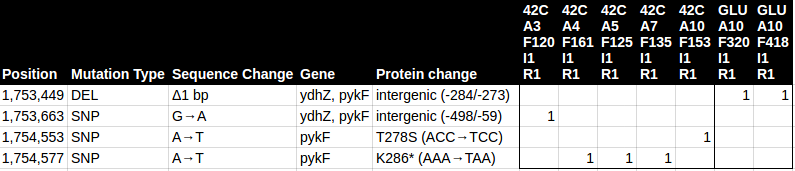
\includegraphics[width=\textwidth]{pykF_shared_enrich_mut.png}
  \label{fig:pykF_shared_enrich_mut}
\end{figure}

\begin{figure}[h!]
  \caption{Shared \textit{hns/tdk} \textit{enrichment} mutations.}
  \centering
  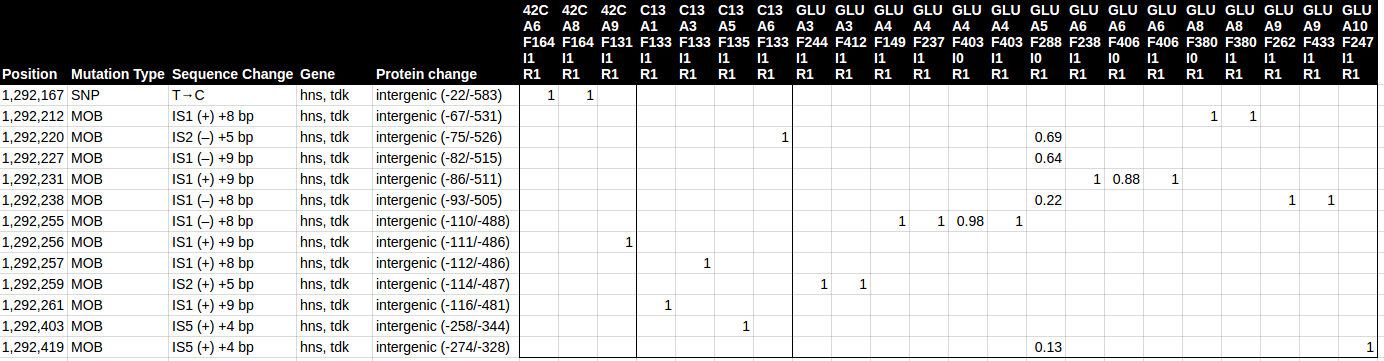
\includegraphics[width=\textwidth]{hns_tdk_shared_enrich_mut.png}
  \label{fig:hns_tdk_shared_enrich_mut}
\end{figure}

\begin{figure}[h!]
  \caption{Shared \textit{rpoB} \textit{enrichment} mutations.}
  \centering
  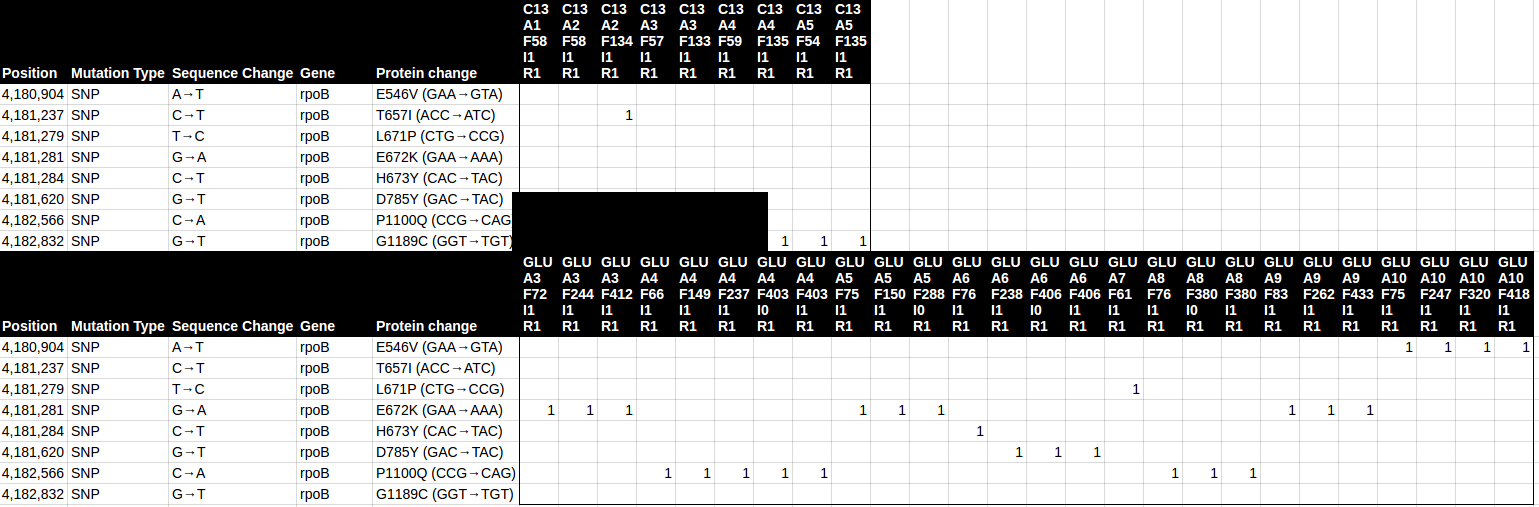
\includegraphics[width=\textwidth]{rpoB_shared_enrich_mut.png}
  \label{fig:rpoB_shared_enrich_mut}
\end{figure}

\begin{figure}[h!]
  \caption{Shared \textit{rpoC} \textit{enrichment} mutations.}
  \centering
  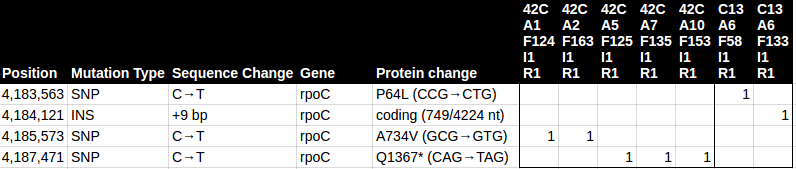
\includegraphics[width=\textwidth]{rpoC_shared_enrich_mut.png}
  \label{fig:rpoC_shared_enrich_mut}
\end{figure}

\begin{figure}[h!]
  \caption{Shared \textit{fixating} \textit{rpoB} alleles.}
  \centering
  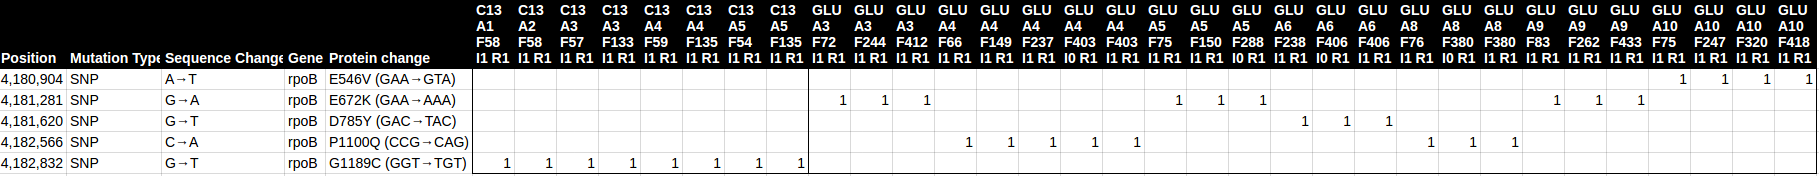
\includegraphics[width=\textwidth]{shared_fixating_rpoB.png}
  \label{fig:shared_fixating_rpoB}
\end{figure}

\begin{figure}[h!]
  \caption{Shared \textit{fixating} \textit{rph} and \textit{rph/pyrE} alleles.}
  \centering
  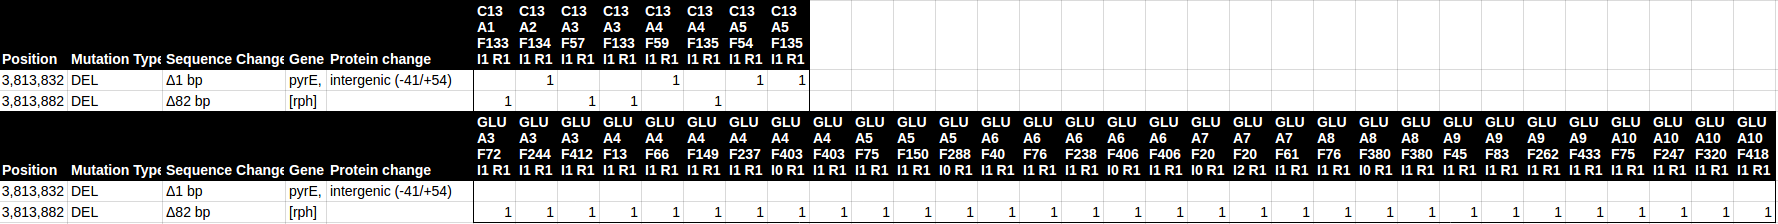
\includegraphics[width=\textwidth]{shared_fixating_rph-pyrE.png}
  \label{fig:shared_fixating_rph-pyrE}
\end{figure}

Throughout the entire ALE experiment database, only two \textit{fixating} alleles were shared among multiple experiments, show in Figures \ref{fig:shared_fixating_rpoB} and \ref{fig:shared_fixating_rph-pyrE}. All of the shared \textit{fixating} alleles were between the C13 and GLU ALE experiments. The GLU and C13 ALE experiments were in fact very similar in that the experiments were designed to select for growth rate, where C13 only differed in the isotope of the carbon source provided. These shared fixations therefore confirm the conclusion of the C13, that the C13 carbon source does not significantly affect the host metabolism and therefore enabled the evolutions of the C13 and GLU experiment to follow a significantly similar track.

\chapter{Summary and Conclusion}

%This type of reporting has been automated in ALE Analytics as the \textit{Mutations} report. This automated report generation along with automated analysis implemented within this platform can save experimentalists weeks of time in manually organizing mutational data and avoid human error in finding significant mutations. Additionally, experimentalists can now expand their ALE experiment sample sets to gain higher mutational resolution in their evolutions beyond any previous limit imposed by the time necessary to organize such data.

% * <pphaneuf@eng.ucsd.edu> 2016-08-15T03:48:44.482Z:
%
% Talk about why population samples conferred an advantage over only using clonal samples.
%
% ^ <pphaneuf@eng.ucsd.edu> 2016-08-16T17:38:45.092Z:
%
% This is detailed in the GLU paper.
%
% ^.
% * <pphaneuf@eng.ucsd.edu> 2016-08-15T16:20:43.689Z:
%
% Talk about the fixating mutation acsending filter, though currently is broken.
%
% ^.
% * <pphaneuf@eng.ucsd.edu> 2016-09-02T17:49:47.719Z:
%
% Conclusion of paper was how similar the key mutations are between the ALEs of this experiment and that of GLU. The evaluation for this paper can therefore have 2 stages, (1) ensuring we're picking up on the same mutations as those called out within the C13 paper, (2) compare the key mutations found (fixated or enriched) between GLU and C13 and describe the matching ALE Analytics key mutations between  both projects.
%
% ^.

%% APPENDIX
\appendix

%% END MATTER
% \printindex %% Uncomment to display the index
% \nocite{}  %% Put any references that you want to include in the bib 
%               but haven't cited in the braces.
\bibliographystyle{alpha}  %% This is just my personal favorite style. 
%                              There are many others.
%\setlength{\bibleftmargin}{0.25in}  % indent each item
%\setlength{\bibindent}{-\bibleftmargin}  % unindent the first line
%\def\baselinestretch{1.0}  % force single spacing
%\setlength{\bibitemsep}{0.16in}  % add extra space between items
\bibliography{template}  %% This looks for the bibliography in template.bib 
%                          which should be formatted as a bibtex file.
%                          and needs to be separately compiled into a bbl file.
\end{document}

